\documentclass[electronic]{kthesis}

%%%%%%%%%%%%%%%%%
%%%% PACKAGES %%%
%%%%%%%%%%%%%%%%%
\usepackage[utf8]{inputenc}
\usepackage[swedish,english]{babel}
\usepackage{csquotes}
\usepackage{enumitem}
\usepackage{caption}   % to align the table caption to the right/left
\usepackage{lscape}
\usepackage{hyperref}  %for references
\usepackage{amsmath,mathrsfs}
\usepackage{amssymb}  % assumes amsmath package installed
\usepackage{epstopdf}
\usepackage{subfig}
% \usepackage{cite}
\usepackage[
  style=ieee,
  sorting=none,
  sortcites,
  hyperref,
  mincitenames=1,
  maxcitenames=2,
  maxbibnames=10,
  minbibnames=1,
  citestyle=numeric-comp, % for [1, 2] instead of [1], [2]
  backend=bibtex
]{biblatex}
\bibliography{Refs.bib,bibliography/bibliography.bib}

% included papers
\DeclareBibliographyCategory{thesispapers}
\addtocategory{thesispapers}{Olguin:DemoScaling2018}
\addtocategory{thesispapers}{Olguin:EdgeDroid2019}
\addtocategory{thesispapers}{Olguin:ImpactWCA2021}
\addtocategory{thesispapers}{CLEAVE2022}


\usepackage{hyperref}
\usepackage{graphicx}
\usepackage{bm}	%Command \bm{make bold}
\usepackage{algorithm}
\usepackage{algpseudocode}
\usepackage{algpascal}
\usepackage{multicol}
\usepackage[x11names]{xcolor}
\usepackage{lipsum}
\usepackage[printonlyused]{acronym}

\usepackage{tikz}
\usetikzlibrary{tikzmark,calc,decorations.pathreplacing}
\newcommand{\Depth}{2}
\newcommand{\Height}{2}
\newcommand{\Width}{2}

\renewcommand{\labelitemi}{\textcolor{IndianRed3}{\bfseries\textbullet}}


%%%%%%%%%%%%%%%%%%%%%%%%%%%%%%%%%%%%%%%
%%%%%%%%% Document starts here %%%%%%%%
%%%%%%%%%%%%%%%%%%%%%%%%%%%%%%%%%%%%%%%
\begin{document}

%%%%%%%%%%%%%%%%%%%%%%%%%%%%%%%%%%%%%%%%%%
%%%%%% First and second pages %%%%%%%%%%%%
%%%%%%%%%%%%%%%%%%%%%%%%%%%%%%%%%%%%%%%%%%
\title{ Thesis Title }
\subtitle{\textbf{sub-title}}
\author{Manuel {Olguín Muñoz}}
\date{\today}
\thesistype{Doctoral Thesis}
\imprint{Stockholm, Sweden, \the\year{}}
\examen{Teknologie doktorexamen i elektroteknik}
\disputationsdatum{fredagen den 18 januari 2020 klockan 14.00}
\disputationslokal{Sal F3, Lindstedtsvägen 26, Kungliga Tekniska Högskolan, Stockholm}
\publisher{Universitetsservice US AB}
\address{%
	KTH Royal Institute of Technology\\%
	School of Electrical Engineering and Computer Science\\%
	Division of Information Science and Engineering\\%
	SE-10044 Stockholm\\%
	Sweden%
}
\isbn{ISBN 100-}
%\issn{ISSN XXX} % No longer used at KTH
\trita{TRITA-EECS-AVL-2020:4}
\kthlogo{KTHLogo}

% Create title page using info above
\maketitle

\frontmatter % Pages i, ii, iii, iv, v etc.

\chapter[Abstract]{}

%%%%%%%%%%%%%%%%%%%%%%%%%%%%%%%%%%%
%%%%%%%%%%% ABSTRACT %%%%%%%%%%%%%%
%%%%%%%%%%%%%%%%%%%%%%%%%%%%%%%%%%%
\begin{abstract}
\noindent \lipsum[1]

\end{abstract}

\bigskip \bigskip \bigskip \bigskip \bigskip

\setlength{\leftskip}{0.3 cm} \textbf {Keywords:} Lorem, Ipsum, Dolor, Sit, Amet

%%%%%%%%%%%%%%%%%%%%%%%%%%%%%%%%%%%%%%%%
%%%%%%%% SWEDISH ABSTRACT %%%%%%%%%%%%%%
%%%%%%%%%%%%%%%%%%%%%%%%%%%%%%%%%%%%%%%%
\newpage
\selectlanguage{swedish}
\begin{abstract}
\noindent \lipsum[1]
\end{abstract}
\selectlanguage{english}
\nocite{
    olguinmunoz2018demoscaling,
    olguinmunoz2019edgedroid,
    olguinmunoz2021impact,
    olguinmunoz2022cleave,
    olguinmunoz2022ainur,
    olguinmunoz2023realistic
}

\printbibliography[
    heading=bibintoc,
    title={List of Papers},
    category=thesispapers
]
\todo[inline]{Fix titlecase!!}
%%%%%%%%%%%%%%%%%%%%%%%%%%%%%%%%%%%%%%%
%%%%%%%% ACKNOWLEDGMENT %%%%%%%%%%%%%%%
%%%%%%%%%%%%%%%%%%%%%%%%%%%%%%%%%%%%%%%
\chapter{Acknowledgements}
\epigraph{La educación es, tal vez, la forma más alta de buscar a Dios.}{\emph{Gabriela Mistral}}
\glsresetall%

There are many, many people I owe gratitude to for making this dissertation possible.
I would like to begin by thanking my supervisor, Prof. James Gross.
This dissertation would not have been possible without his guidance and motivation during this long process.
His supervision opened doors that I had never imagined would open for me, and his dry German humor has certainly helped cheer me up whenever I was overwhelmed by some deadline.
Above all, I would like to thank James for his patience and understanding whenever I encountered difficulties, and for the flexibility he has afforded me in completing this Ph.D.

I would like to express my deepest gratitude to Prof. Mahadev ``Satya'' Satyanarayanan, for welcoming me repeatedly, over long periods of time, as a visiting researcher at \gls{CMU}.
Likewise, I'm deeply indebted to Prof. Roberta ``Bobby'' Klatzky of \gls{CMU} for the many helpful and insightful discussions, for introducing me to the field of Human-Computer Interaction, and for always greeting me with a warm smile.
Both Satya's and Bobby's tremendous experience and generosity have been invaluable, and their guidance and advice have certainly shaped my work for the better.

I would also like to thank everybody involved with the defense of this thesis.
I am very grateful to Prof. Yu Xiao of Aalto University, for agreeing to act as my dissertation opponent.
My dissertation defense will certainly benefit greatly from her expertise and insights.
I would like to extend my sincere thanks to my grading committe, consisting of Prof. Ana Aguiar (Universidade do Porto), Prof. Per Gunningberg (Uppsala Universitet), and Prof. Klaus Wehrle (\gls{RWTH}), for investing time and effort into reading and grading this dissertation.
Special thanks also go to Prof. Markus Flierl of \pgls{KTH} for advance-reviewing this dissertation, and to Prof. Mats Bengtsson, also of \pgls{KTH}, for agreeing to act as chairperson for the defense.

Moreover, I extend my thanks to my co-authors and colleagues.
To Samie Mostafavi, Vishnu N. Moothedath, and Neelabhro Roy at \pgls{KTH}, for always being willing to engage in interesting discussions, but also for generally being fun to be around.
And to Dr. Jaya Prakash (IMDEA Networks Institute), Dr. Junjue Wang (\gls{CMU}), and Dr. Padmanabhan ``Babu'' Pillai (\gls{CMU}) for enriching my research with their interesting insights.

I am very lucky and grateful that I got to stay at both \pgls{KTH} and \gls{CMU}, and I would like to thank everyone who made these spaces welcoming and engaging.
A big thank you goes out to my colleagues (both current and former) at the division of \gls{ISE} for all those fun lunches at Restaurang Q, Cypern, and SysterOBror over the years, which always helped to break the monotony of the days.
This includes but is not limited to Samie, Vishnu, Neel, Sahar, Antonios, Germán, Boules, Baptiste, Håkan, Pol, Marie, Wendi, and Sebastian.
I would additionally like to extend a special thank you to Dr. Sebastian Schiessl, for ``taking me under his wing'' when I first arrived at \gls{ISE} and acting as a sort of mentor during my first moths.
Likewise, I extend my gratitute to Gerd Fransson, for greeting me with a huge smile every morning the years our offices faced each other and cheering up my days with her wholesome energy.
I also thank Prof. Joakim Jaldén for giving me the opportunity to act as his teaching assistant.
Another big thank you goes out to everyone (current and former) at Satya's group at \gls{CMU}, for always welcoming me with open arms and treating me like one of them whenever I was visiting.
This includes but is not limited to Junjue, Tom, Roger, Shilpa, Jan, Edmond, Jim, Babu, and Zhuo.
I will always remember our Monday morning talks and Friday lunch outings dearly.

Furthermore, I would like to extend my sincere thanks to Prof. Sandra Céspedes, of Universidad de Chile and Concordia University, for her guidance and urging to embark on this journey towards a Ph.D., and for always being willing to offer help and advice.
Likewise, I'd like to thank Prof. Javier Bustos, of Universidad de Chile and NIC Chile Research Labs, for giving me the opportunity many years ago to first get into distributed systems research.
Also, I'd like to extend my gratitude to Prof. José Miguel Piquer, of Universidad de Chile, for taking me as his ``long-distance'' teaching assistant and allowing me to give back to my \emph{alma mater} from across the ocean.
A very special thanks goes out to Prof. Jérémy Barbay of Universidad de Chile and Universidad de Concepción, for being both a mentor and a friend since the day I took his course on Android programming as an undergraduate student.
I am deeply appreciative of the fact that although our interactions these last few years have been sporadic at best, I can always reach out to him for help and advice when I need them.

\medskip

This dissertation would not have been possible without the help and support of my family.
First and foremost, I would like to thank the love of my life and wife~\footnote{\emph{Future-wife} at the time of writing, but \emph{wife} at the time of the defense of this thesis!}, Andresa.
I could not have done this without her companionship and love.
I am eternally grateful for her unconditional support over difficult periods of time and over tremendous distances while we were living apart, and for making every day we spend together amazing.

I am also deeply grateful to my parents, Gabriel and Valeria, for always encouraging my curiosity and my drive to learn and discover.
They have been my rocks, my pillars, since the day I was born, and I am proud to be their son.
A big thank you goes out to my sister, Paola, as well.
Although we sometimes get on each other's nerves, she has always been there for me and supported me, and I could not have asked for a better sister.
Likewise, I extend my deepest gratitude to everyone in my immediate and extended family who have given me support and love over the years, including but not limited to my paternal grandparents, Manuel and María Yolanda, my maternal grandparents, Caupolicán and María Aura, my uncle Mauricio, his wife Marylen, their daughter Amanda, and everybody else.
I would like to make a special mention to my late grandfather, Caupolicán ``Poli'' Muñoz, who always inspired and fanned the flames of academic curiosity in me.
I hope he would have been proud seeing how far I have come.
Another special mention goes to my uncle Manuel, who graciously took me in and gave me a place to stay at the first few months of my Ph.D. studies.

I would also like to thank all of my friends who have made this long, ardous journey more amenable.
I would particularly like to thank everyone I met through Tartan Salsa, including, but not limited to, Andresa, Jennifer, Alyson, Kuai-Kuai, Carmen, Moataz and Nora, Eric, and many others.
They made Pittsburgh feel like home, even before I finally moved there permanently in 2022.
I also want to thank Ann-Charlotte in Stockholm, for always being so kind, so considerate, and so much fun to be around.
Further, I am deeply grateful to my friends in Chile who have remained a source of support, even though we only get to see each other once a year when I visit.
This includes, but is not limited to, Juan Pablo, Fernanda, Diego, Camila, George, Patricio, Kevin, Pablo, and many others.
Yet another special mention goes to Diego's family, who have always treated me as one of their own.

Finally, I would be remiss in not mentioning my pets and animal friends who have provided me with love and warmth during these years.
I thank my dogs, Aros and Skatt, who I sadly had to leave behind in Chile with my sister, but who still greet me with enthusiastically wagging tails whenever I visit.
And I thank my cats, Mochi and Tiramisú, who, although have only been in my life for about a year, have sweetened and made much more bearable the long days and nights I have spent writing this dissertation.

\bigskip

\noindent{}Manuel Olguín Muñoz\\
Pittsburgh, May 2023
%%%%%%%%%%%%%%%%%%%%%%%%%%%%%%%%
%%%%%%%% ACRONYMS %%%%%%%%%%%%%%
%%%%%%%%%%%%%%%%%%%%%%%%%%%%%%%%
\chapter{Acronyms}
\begin{acronym}
    \acro{CPS}{Cyber-Physical System}
    \acro{NCS}{Networked Control System}
    \acroindefinite{NCS}{an}{a}
    \acro{LAN}{Local-Area Network}
    \acro{WLAN}{Wireless Local-Area Network}
    \acro{KPI}{Key Performance Indicator}
    \acro{WPAN}{Wireless Personal Area Network}
    \acro{CSMA/CD}{Carrier-Sense Multiple Access with Collision Detection}
    \acro{CLEAVE}{ControL bEnchmArking serVice on the Edge}
    \acro{OS}{Operating System}
    \acro{UDP}{User Datagram Protocol}
    \acro{TCP}{Transmission Control Protocol}
    \acro{RMS}{Root Mean Square}
    \acro{RTT}{Round-Trip Time}
    \acro{CI}{Confidence Interval}
    \acro{AP}{Access Point}
    \acro{API}{Application Programming Interface}
    \acro{SSF}{Swedish Foundation for Strategic Research}
    \acro{TECoSA}{Trustworthy Edge Computing Systems and Applications}
    \acro{ABC}{Abstract Base Class}
    \acroplural{ABC}[ABCs]{Abstract Base Classes}
    \acro{URL}{Uniform Record Locator}
    \acro{AWS}{Amazon Web Services}
    \acro{EC2}{Elastic Compute 2}
    \acro{AMI}{Amazon Machine Image}
    \acro{SSH}{Secure Shell}
    \acro{IP}{Internet Protocol}
    \acro{VPN}{Virtual Private Network}
    \acro{NAT}{Network Address Translation}
    \acro{NTP}{Network Time Protocol}
    \acroindefinite{NTP}{an}{a}
    \acro{SDR}{Software-Defined Radio}
    \acroindefinite{SDR}{an}{a}
    \acro{VLAN}{Virtual Local-Area Network}
    \acro{APT}{Advaced Packaging Tool}
    \acro{LTE}{Long-Term Evolution}
    \acro{SSID}{Service Set Identifier}
    \acro{EPC}{Evolved Packet Core}
    \acro{UE}{User Equipment}
    \acro{eNodeB}{Evolved Node B}
    \acro{DNS}{Domain Name System}
    \acro{MNIST}{Modified National Institute of Standards and Technology}
    \acro{HTTP}{Hyper-Text Transfer Protocol}
    \acroindefinite{HTTP}{an}{a}
    \acro{YAML}{YAML Ain't Markup Language}
    \acro{O-RAN}{Open Radio Access Network}
    \acro{FOSS}{Free and Open Source Software}
    \acro{COSMOS}{Cloud enhanced Open Software defined MObile wireless testbed for city-Scale deployment}
    \acro{OMF}{ORBIT Management Framework}
    \acro{POWDER}{Platform for Open Wireless Data-driven Experimental Research}
    \acro{COTS}{Commercial Off-The-Shelves}
    \acro{RF}{Radio-Frequency}
    \acro{VM}{Virtual Machine}
    \acro{REST}{REpresentational Sate Transfer}
    \acro{OS}{Operating System}
    \acro{MaaS}{Metal-as-a-Service}
    \acro{OEDL}{\ac{OMF} Experiment Description Language}
    \acro{RSpec}{Resource Specification}
    \acro{LXC}{LinuX Containers}
    \acro{MEC}{Mobile Edge Computing}
    \acro{USRP}{Universal Software Radio Peripheral}
    \acro{OAI}{OpenAirInterface}
    \acro{NR}{New Radio}
    \acro{FPGA}{Field-Programmable Gate Array}
\end{acronym}

\mainmatter % Pages 1, 2, 3...

\tableofcontents*{}
\part{Summary}
\chapter{Introduction}\label{chap:introduction}

\todo[inline]{
    Introduction here. Why do we need this work?
}

\todo[inline]{
    Reorganize EdgeDroid, Cleave, Ainur, together.

    Pull in multi-loop results for EdgeDroid?

    Think about experiments.
}

\section{Summary of the key contributions of this thesis}

This thesis presents three core contributions to the existing body of research in edge computing, as well as a number of secondary ones.
Firstly, we introduce a methodological approach to studying system responsiveness versus resource consumption trade-offs in edge-bound feedback-loop systems such as \gls{WCA} and \gls{NCS}.
This approach is based on the emulation of the client-side workload, while maintaining the \emph{real} server-side process as well as network stack.
We validate this methodology by example, presenting implementations of its application in the context of \gls{WCA} and \acp{NCS}, and introduce a software framework for the orchestration of the edge computing testbeds necessary for its implementation.

Secondly, we present a deeper exploration of this methodology for \gls{WCA} and introduce the first ever model for the end-to-end emulation of human timing behavior in \gls{WCA}.
This model is built from a thorough characterization of these behaviors, the data for which we obtain from a comprehensive human-subject study.

Finally, as an extension and application of our first and second contributions, we explore the implications of our methodology and human user model on the optimization potential of \gls{WCA} deployments.
In particular, we study the sampling and energy consumption behaviors of these systems with and without considering realistic human behavior.
We conclude that significant improvements can be achieved through the use of our human user model.

\subsection{Overview of each included paper}

\cref{paper:olguinmunoz2018demoscaling,paper:olguinmunoz2019edgedroid,paper:olguinmunoz2022cleave,paper:olguinmunoz2022ainur} introduce and discuss this methodology and the necessary tools for its implementation.
\cref{paper:olguinmunoz2018demoscaling} presents a short, high level overview of this methodological approach as applied to \gls{WCA}, making very straightforward assumptions about human behavior in \gls{WCA} applications.
\cref{paper:olguinmunoz2019edgedroid} extends the discussion from \cref{paper:olguinmunoz2018demoscaling}, providing more details on the implementation of the necessary measurement framework and the tooling employed.
This work presents the first empirical results obtained with our methodological approach, providing thus an initial validation of its utility for research.
\cref{paper:olguinmunoz2019edgedroid} also discusses in detail the assumptions that were made about human behavior and reactions.
We assume in these works a human which is impervious to poor system performance, and suffers no annoyance, fatigue, frustration, nausea or other shortcomings of real human users.
The result is a model of a user who responds in a precisely reproducible and deterministic manner to the same system stimulus every time.

\cref{paper:olguinmunoz2022cleave}, on the other hand, presents a discussion on the implementation of this methodology for \acp{NCS}.
As discussed above, these applications are similarly difficult as \gls{WCA} to benchmark (in particular at scale on multi-tenant systems) due to their client-side complexity, but in particular because of their often extreme sensitivity to latency.
\todo[inline]{More argumentation or refer to previous section.}
We apply thus in this work our methodology to \gls{NCS} through the implementation of a tool for the emulation and subsequent deployment of these systems on edge computing infrastructure.
This tool allows us to both emulate the physical components of a relatively simple control system plant and deploy real algorithms for its control.
The software acts as a middleware which abstracts away the network from the development of these workloads, allowing for quick prototyping and deployment.
This work also showcases the scalability and flexibility of our approach, allowing us to deploy scenarios with a large number of loops without the need for domain-specific hardware.

\cref{paper:olguinmunoz2022ainur} presents a tangential contribution.
It introduces the software framework used in \cref{paper:olguinmunoz2023realistic,paper:olguinmunoz2022cleave} for the orchestration of the edge computing testbeds on which the developed tools were deployed.
This framework represents an ancillary contribution, crucial for the research presented in these works.
Without it, the experimental approach described in these works would not have been feasible.

Next, in \cref{paper:olguinmunoz2021impact,paper:olguinmunoz2023realistic} we delve deep into the implementation of our methodology for \gls{WCA}, as well as study its implications for optimization of these systems.
Although the above approach to human behavior in \gls{WCA} discussed represents a useful initial approximation, it is nonetheless not a realistic model of it.
In \cref{paper:olguinmunoz2021impact} we therefore take the first major step towards such a model, presenting a deep characterization of human behavior in these applications.
We develop this characterization through a human subject study with a cohort of \num{40} participants who were asked to interact with an instrumented \gls{WCA} application.
System responsiveness is altered in real-time during each execution of the task, and we record participants' reactions by measuring task- and system-related metrics, as well as biometrics from sensors placed on their bodies.
Participants were also asked to fill out two personality indicator questionnaires, allowing us to later correlate individual personality traits and measured reaction to changes in system responsiveness.

\cref{paper:olguinmunoz2023realistic} then concludes this line of work, building upon the insights and data obtained in \cref{paper:olguinmunoz2021impact} to develop the first ever data-driven model of human timings for \gls{WCA}.
The model is validated against previously obtained results, both through simulated, controlled executions and deployments on a real edge computing testbed.
This work also explores potential implications of this model for \gls{WCA} system optimization potential, particularly in the domains of energy consumption and sampling strategies.

\section{Structure of this thesis}

\todo[inline]{This thesis is structured as follows.}
\chapter{Key contributions and results}\label{chap:contributions}

\section{A methodology for the study of feedback-loop systems in Edge Computing}\label{summary:methodology}

\begin{figure}
    \centering
    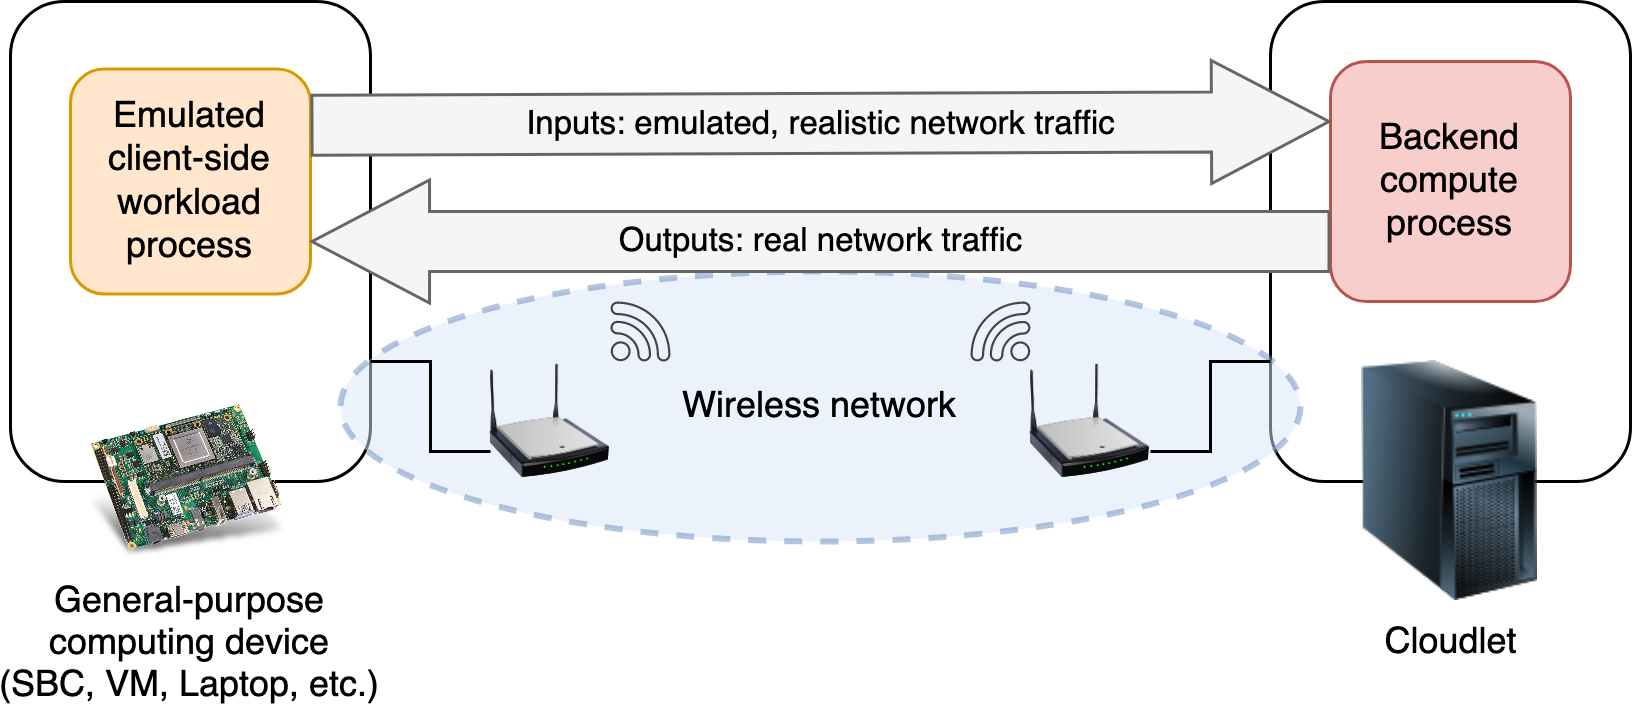
\includegraphics[width=.8\textwidth]{Figs/methodology.png}
    \caption{%
        Overview of the proposed methodology for the study of feedback-loop systems on edge computing infrastructure.
        The  client side of the system is replaced with an emulation executed on a general-purpose computing device.
        The backend/server side of the system along with the network remain unchanged.
    }\label{fig:methodology}
\end{figure}

As discussed above, benchmarking infrastructures for edge-bound applications featuring feedback-loops is challenging, in particular when dealing with applications with high sensitivity to latency (such as \ac{NCS}) or with human involvement (such as \ac{WCA}).
In the following, we introduce our methodological framework for tackling this challenge.

A general overview of our methodology is illustrated in \cref{fig:methodology}.
It is based on the core idea of executing an emulation of the target workload on top of the real hardware on which it is to be deployed.
We replace the client side of the system with a realistic emulation of the desired behaviors; this emulation is implemented in software deployed on \ac{COTS} general-purpose computing devices.
The backend side and the network are not changed.

Two main arguments drive this approach.
One, the difficulty of scaling the number of clients in these systems in a research context.
The systems we target exhibit a centralized nature in which a potentially large number of clients offload computation to a single central compute node.
The client-side component of the applications of interest for this research is often complex to scale, either due to the involvement of humans (as in the case of \ac{WCA}) or due its cyber-physical nature (in \acp{NCS}).
Emulating this component reduces this complexity by moving it into the software domain, allowing for easier scaling through the use of cheap, general-purpose hardware such as single-board computers (e.g. Raspberry Pis, Beaglebones, etc.).

And two, it maintains the realism of the most complex parts of the system.

\todo[inline]{Fix and finish}

In the following, we will discuss the initial implementation of this methodology to two different classes of applications.
We first discuss the methodology in the context of a human-in-the-loop application, \acl{WCA}, in section \cref{ssec:methodology:wca}.
Then, in \cref{ssec:methodology:ncs}, we present an exploration into it's utility for the study of \acf{NCS}.


\subsection{Applying the methodology to \acs{WCA}}\label{ssec:methodology:wca}

\begin{figure}
    \centering
    \begin{subfigure}[b]{.47\textwidth}
        \centering
        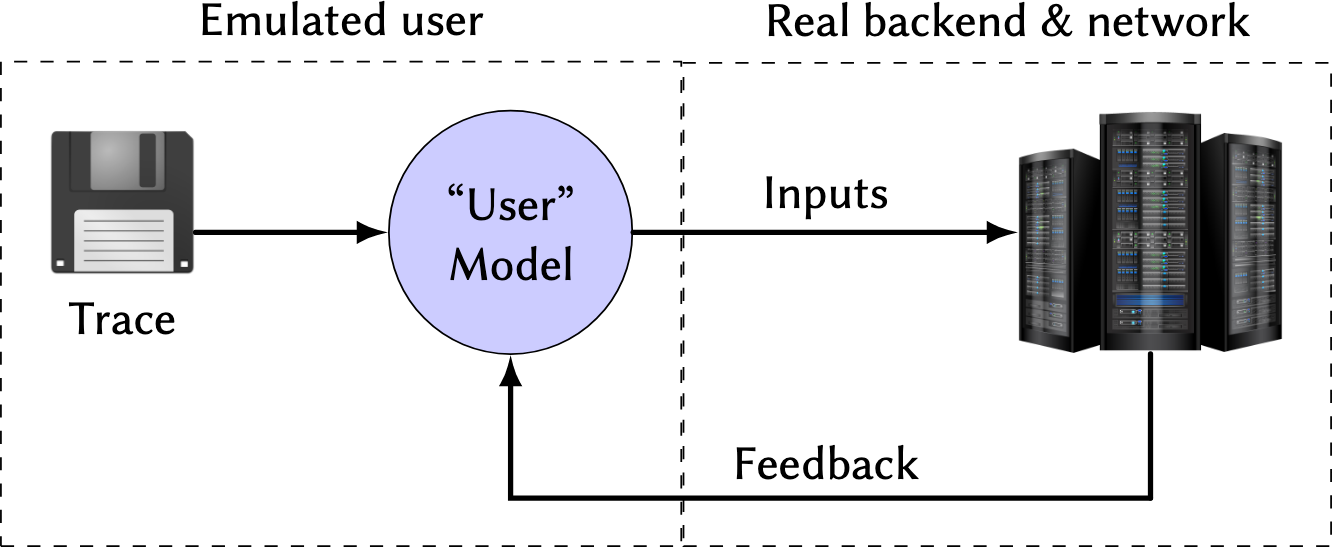
\includegraphics[width=\textwidth]{Figs/trace_edgedroid.png}
        \caption{%
            High level conceptual design of our methodology for \ac{WCA}.
            We replace the human by a trace-driven emulation.
            This allows us to maintain realism in inputs sent over the network to the compute process on the backend, while simplifying the design of the client software.
        }
    \end{subfigure}
    \hfill
    \begin{subfigure}[b]{.47\textwidth}
        \centering
        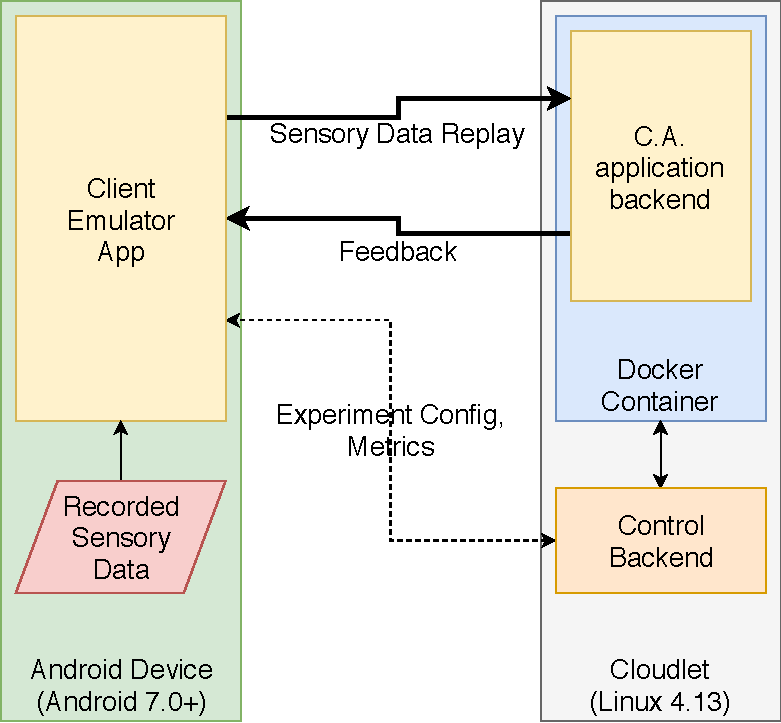
\includegraphics[width=\textwidth]{publications/2018DemoScalingOnTheEdge/img/TraceReplay_GenArch}
        \caption{%
            Architectural overview of the EdgeDroid \num{1.0} tool.
            The ``client emulator app'' implements the aforementioned user model together with the required networking functionality to connect to a \ac{WCA} backend running on a cloudlet.%
            }
    \end{subfigure}\\
    \medskip
    \begin{subfigure}[t]{\textwidth}
        \centering
        \adjustbox{scale=0.7}{
            \begin{tikzpicture}[align=center,
            node distance=.5cm and 1.5cm,
            every initial by arrow/.style={-{Latex[length=2mm]}}]
            % Place nodes              
            \node [initial, state, minimum size=6em, initial text=] (play) {Play};               
            \node [state, above right=of play, minimum size=6em] (change) {Change\\step};
            \node [state, below right=of play, minimum size=6em] (rewind) {Rewind};
            \node [state, accepting, above right=of rewind, minimum size=6em] (shutdown) {Shutdown};
            
            % Draw edges
            \path[draw, -{Latex[length=2mm]}]
            (play) edge [bend right=20] node[left] {Step done} (rewind)
            edge [bend left=20] node[left] {Got feedback\\(\emph{positive})} (change)
            edge [out=140,in=220,looseness=6] node[left] {Step\\not done} (play)
            
            (change) edge [bend left=20] node[right] {Step changed} (play)
            edge [bend left=20] node[right] {All steps done} (shutdown)
            
            (rewind) edge [bend right=20] node[right] {Rewound} (play)
            edge [bend right=20] node[right] {Too many rewinds} (shutdown);
            
            \end{tikzpicture}
        }
        \caption{State diagram of the user model governing the replay of the pre-recorded trace at runtime. This model approximates the behavior of an ``ideal'' human, one that is patient and makes no mistakes.}\label{fig:usermodel}
    \end{subfigure}
    \caption{%
        Overview of our first implementation of the methodology for \ac{WCA}.
    }\label{fig:edgedroid1:trace}
\end{figure}

We first introduce our methodology in \cref{paper:olguinmunoz2018demoscaling,paper:olguinmunoz2019edgedroid}.
The former corresponds to an extended abstract paper which discusses a high level overview of our approach; the latter presents a deeper, more complete discussion about the implementation together with some first experimental results.

The overall goal of these papers is to explore this methodological approach as applied to \ac{WCA}.
As discussed in \cref{chap:introduction}, the main challenge to benchmarking \ac{WCA} --- and other ``human-in-the-loop'' applications on the edge --- concerns the involvement of human beings in their operation.
Humans are unreliable, and, perhaps more importantly, hard to scale.
\todo[inline]{More reasons}

The implementation of the client-side emulation necessary for our methodology follows in these works a trace-based design.
We introduce a tool, \emph{EdgeDroid \num{1.0}}, which replays a pre-recorded trace of sensory inputs to the original \ac{WCA} backend.
The tool is implemented in Android, allowing for its easy deployment on the same kind of \ac{COTS} mobile devices on which real \ac{WCA} applications are intended to run in the future.
Furthermore, this tool is instrumented, allowing us to collected a multitude of system-level metrics at runtime which can then be analyzed.
On the other hand, the trace in question corresponds to a pre-recorded sequence of sensory inputs obtained from a real execution of the \ac{WCA} by a human volunteer.
The trace is recorded in a near-ideal setting, such that it does not include either human mistakes or segments with degraded system responsiveness.
Once recorded, the trace is manually segmented into the logical component steps of the task, and these are replayed in sequence back to the backend by the EdgeDroid tool.

We opt for a trace-based approach for our first implementation of the methodology for \ac{WCA} for three key reasons.
The first of these is the level of realism if affords in terms of the payloads sent over the network and, in particular, processed by the backend.
Using a trace ensures that the same computation is performed on the edge as if a human was involved, while also ensuring a reproducible application execution path.

The second is simplicity, as such an approach does not require complex modeling of human behavioral patterns, merely the observation and recording of them.
Compatible traces can be easily obtained simply by instrumenting existing \ac{WCA} client applications to record all captured inputs.

The final advantage corresponds to extensibility.
As long as the tasks belong to the same category of \ac{WCA} applications (in this case, step-based cognitive assistance), using a trace makes extending the tool to different tasks merely a matter of recording a new trace.

\todo[]{}



reproducible and comparable workload, we use a trace-based design for the client-side emulation.
.

To then use the trace for reproducible experiments, we introduce a benchmarking suite which can replay the trace to the original application.
This results in the same computation to be performed on the edge as if a human was involved, while also ensuring a reproducible application execution path.
Additionally, the suite is instrumented to collect system level metrics at runtime for posterior analysis.

However, merely replaying the trace is not enough, as disparities between system responsiveness at recording versus replay time can cause the trace so drift out of synchronization with the current state of the system.
Thus, we introduce here the concept of a human user model which is able to adapt its behavior in a realistic manner based on the current responsiveness of the system by systematically controlling the replay of the trace.
The initial approximation we introduce, illustrated in \cref{fig:usermodel}, here is that of a human that is patient and does not make mistakes, and any error message received from the application backend is ignored.
The trace is preprocessed into segments that correspond to individual steps of the \ac{WCA} application; this is performed manually as a preparation step.
The user model then replays each segment in order; whenever feedback corresponding to a change of step is received from the \ac{WCA} backend, the user model transitions to the next segment in the trace, no matter whether the current segment has been replayed out completely or not.
On the other hand, if no step transition feedback has been received at the end of the current trace segment, the model rewinds the trace a $\tau$ seconds and tries again.
To avoid infinite loops, where the application is stuck on a step forever, we have a maximum number of possible rewinds, after which the application shuts down.

\todo[inline]{EdgeDroid paper}



\begin{figure}
    \centering%
    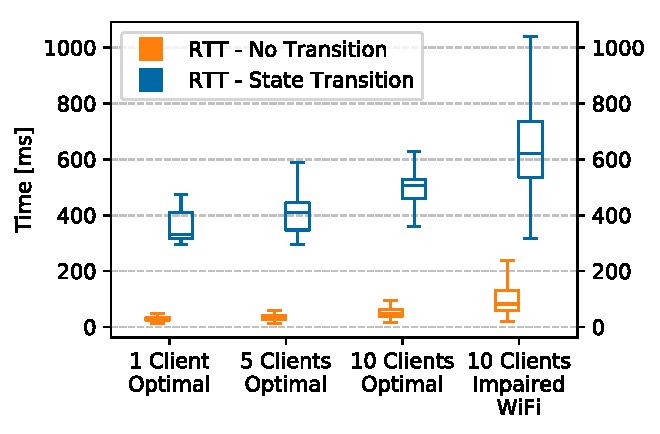
\includegraphics[width=.85\textwidth]{publications/2019EdgeDroid/plots/comparison/nofonts/rtt_fb_vs_nofb}%
    \caption{Comparison of round-trip-times for inputs that triggered a state transition in the task model versus inputs that did not.}%
    \label{fig:comparison:rtt}%
\end{figure}%
\begin{figure}
    \centering%
    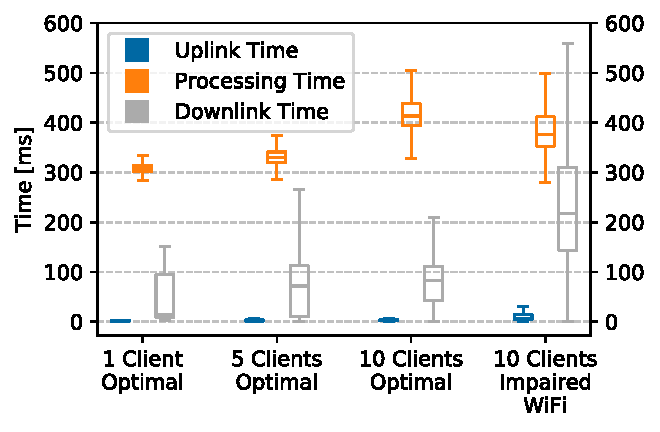
\includegraphics[width=.85\textwidth]{publications/2019EdgeDroid/plots/comparison/nofonts/box_feedback}%
    \caption{Distribution of latency across system components for inputs that triggered a state transition in the task model.}%
    \label{fig:comparison:feedback}%
\end{figure}%
\begin{figure}%
    \centering%
    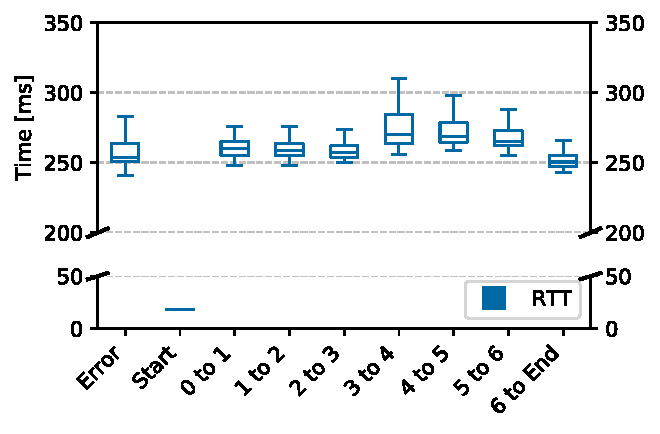
\includegraphics[width=.85\textwidth]{publications/2019EdgeDroid/plots/comparison/nofonts/box_taskstep}%
    \caption{Round-trip-times for input-feedback cycles associated with state transitions in the internal task model for a single client connected over an optimal wireless link.}%
    \label{fig:comparison:tasksteps}
\end{figure}%

The goal of this paper is to provide a methodological approach to studying these latency trade-offs, along with a tool, EdgeDroid 1.0\footnote{We plan to make the EdgeDroid 1.0 benchmarking suite available as Free and Open Source Software and the recorded traces under a Creative Commons License.}, that simplifies the benchmarking of human-in-the-loop applications.
We view EdgeDroid 1.0 to be the very first, and simplest, of a family of tools that will embody increasingly sophisticated and accurate models of user behavior.

Due to the complex nature of the applications and the infrastructure, we opt for experimentally studying the trade-offs in a repeatable and controllable fashion.
This is difficult mainly due to the unpredictable reaction of human users to the feedback from the backend --- a user might very well misinterpret the feedback handed to them.
EdgeDroid 1.0 mimics the operation of human-in-the-loop applications by replaying recorded traces of sensory input.
This sensory information is then processed by the original compute process at the backend, generating feedback.
However, this feedback is not processed by humans, but by a parameterizable model of human reaction.
Through synchronized time tracking at the different processing points of the application, EdgeDroid 1.0 allows for accurate measurements of key performance metrics such as the distribution of delays across the application pipeline.
Analysis of these metrics can be performed down to the individual input sample, allowing us to zoom into the internal model of the application under consideration.
Thus, EdgeDroid 1.0 allows us to illuminate the many latency trade-offs existing at the level of the infrastructure, as well as the level of the application.
It can also be used for debugging and validation, by comparing the expected execution flow of a particular trace with the actual flow during the benchmarking.
To the best of our knowledge, this experimentally-driven benchmarking approach is the first one towards experimental performance characterization and potential optimization of human-in-the-loop applications

\Cref{fig:comparison:rtt} presents a comparison of the total measured round-trip-times (RTTs) both for inputs which caused a state transition and inputs that did not.
Next, \cref{fig:comparison:feedback} shows a comparison of the distribution of latencies across system components for inputs that caused an internal state change in the task model of the application.
We differentiate according to the three main components contributing to latency, namely \emph{uplink} and \emph{downlink transmissions}, and \emph{backend processing}.
Finally, \cref{fig:comparison:tasksteps} depicts the distribution of RTTs for each transition in the internal task model for a single client connected over an optimal wireless link.
These metrics were calculated by recording the measured input-feedback cycle delay corresponding to a change in state within the application.
Thus, for instance, the measurements located at column ``3 to 4'' in the figure correspond to the aggregated round-trip-times for every input-feedback cycle corresponding to a change from state 3 to state 4 within the application task model, for the 100 repetitions of the scenario.

In the following discussion we will refer to inputs which triggered a transition in the task model as \emph{feedback-rich inputs} and those that did not as \emph{feedback-less inputs}.

For the analysis of these results, we will take into consideration the bound of \SI{600}{\milli\second} response time for step-by-step task-guidance derived by the authors of~\cite{Chen:AnEmpiricalStudyOfLatency}.
This bound marks the point after which further delays in the delivery of feedback to the user start to negatively affect user experience, and allows for a straightforward evaluation of the responsiveness of the system.

We will begin our analysis of the experiment results with \Cref{fig:comparison:rtt}.
These results present a stark contrast in the round-trip-times for inputs which cause a state transition versus inputs that do not, with RTTs for the former being up to an order of magnitude greater.
It's worth mentioning though that responses to feedback-less inputs are invisible to the user, and are just included here as a sort of baseline to compare feedback-rich round-trip times with.

We can identify a pair of interesting effects in the scaling of the task-guidance WCA application.
One, scaling behavior for the application seems to be linear with respect to the number of clients.
Two, in the case of the impaired WiFi, the effect on the feedback-rich inputs is very pronounced, with the average of the RTTs for these inputs being over the previously discussed bound of \SI{600}{\milli\second}.

It is worth noting that already at just 10 clients the response times for feedback-rich inputs are very close to the bound.
Looking at this through the lens of a an application developer, it could hint at a need for optimization of the later parts of the application pipeline, since RTTs for inputs which are discarded in the detection stage of the pipeline (i.e.\ feedback-less inputs) are still well below \SI{200}{\milli\second}.

EdgeDroid 1.0 allows researchers to zoom into specific components of the application feedback loop, as exemplified by \cref{fig:comparison:feedback}.
From this figure it is clear that the main component which contributes to latency in the optimal case is the backend processing, further lending credibility to our previous comment on the need for optimization.
Nevertheless, when the link quality decreases, the delays on the downlink start to overshadow the delays on the processing.
Here, the downlink time sometimes almost reaches the ideal bound by itself.
A system designer might then conclude from this that in order to be able to scale the application, their focus needs to be on improving the quality of the wireless link before increasing the processing power on the backend.

Finally, EdgeDroid 1.0 allows even more insights to be gained by homing in to individual steps in a task-guidance WCA. Consider \cref{fig:comparison:tasksteps}.
The figure shows clears spikes in latencies at the transitions from task state 3 to 4 and from task state 4 to 5, which could indicate to the application developer that these specific transitions are ripe for optimization.


\todo[inline]{\cref{paper:olguinmunoz2019edgedroid}}\label{summary:2019edgedroid}

\subsection{Applying the methodology to \acsp{NCS}}\label{ssec:methodology:ncs}

\todo[inline]{\Cref{paper:olguinmunoz2022cleave} implements both the methodology and the tool.}

\begin{figure*}
    \centering
    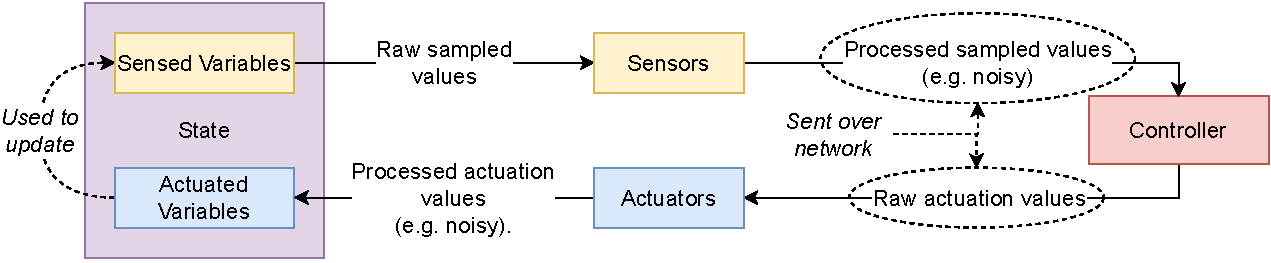
\includegraphics[width=.8\textwidth]{publications/2022CLEAVE/images/CLEAVE_NCS_structure}
    \caption{
        Structure of an emulated \acl*{NCS} in \acs*{CLEAVE}.
    }\label{fig:cleave:ncs:struct}
\end{figure*}

We overcome this issue by proposing a completely virtual plant allowing for unparalleled flexibility in changing the plant model and characteristic features of the experiments.
In this paper, we present the first fully-software-based framework for scalable and repeatable benchmarking of edge-native \ac{NCS}.
As edge computing begins being adopted by industry, more and more variations have begun to appear in literature.
``Near'', ``far'', ``core'', and ``telco'' edge describe variations of the original concept and are becoming ubiquitous in new research.
While the core idea of edge computing is widely accepted as fundamental for pervasive \acp{NCS} in general, understanding the strengths and weaknesses of such different edge concepts is of paramount importance.

Our framework, \ac{CLEAVE}, aims to simplify the repeatable and scalable benchmarking of such systems.
It is fully virtualized, inspired by our previous work on benchmarking human-in-the-loop applications on the edge~\cite{Olguin2019EdgeDroid}.
The tool consists of a benchmarking framework and software development kit for the development of emulated physical systems and softwarized controllers.
These virtual \acp{NCS} can then be deployed on real networks for reparametrizable, repeatable, and reproducible benchmarking of the complete system.

\ac{CLEAVE} is built using \emph{Python 3.8}, making it highly extensible and able to harness the multitude of already existing user libraries.
It is furthermore compatible with container technologies such as \emph{Docker}\footnote{Docker Engine: \url{https://www.docker.com/}}, making it suitable for automated deployment, scaling, and benchmarking on industry-standard edge setups using container orchestration solutions.

In this work, we aimed to tackle this issue through a fully software-based framework for repeatable, reproducible, and easily scalable \ac{NCS} benchmarking with a particular focus on edge deployment.
We argue our approach, \ac{CLEAVE}, embodies a better solution than previous work for a number of reasons:
\begin{enumerate}
    \item Compared to fully physical approaches, such as those used in\ \cite{Baumann2018LowPower} and\ \cite{Cuenca2019UAV}, our approach allows for greater flexibility and scalability.
          The aforementioned approaches rely on specialized and sometimes entirely custom-built physical platforms, and although flexible and cheap approaches such as Zoppi \emph{et al.'s} --- which uses a LEGO-based physical plant --- exist, these still do not reach the level of flexibility afforded by a fully software-based framework.
          Experimenters still need copies of the hardware, making anything other than small-scale setups unfeasible.
          In contrast, our approach requires only general-purpose computing platforms, and can be employed by basically anyone with access to a computer.
          Scalable deployments can in turn easily and cheaply be set up using single-board computers and/or virtual cloud instances.
    \item When compared to simulated approaches such as\ \cite{Ma2019DynamicSched}, \ac{CLEAVE} provides a higher level of realism, in particular with regards to the network segment of the system.
    \item Finally, although it shares much in common with previous emulated approaches such as the one employed in\ \cite{Wang2020VoltageControl}, \ac{CLEAVE} has an advantage by specifically targeting a general-purpose approach using industry-standard, cloud- and edge-native tools and software.
          The tool can easily be deployed and scaled using widely-used frameworks such as Docker Swarm and Kubernetes.
\end{enumerate}

We validate the utility of this tool through an example use case approximating a proposed edge deployment of inverted pendula control loops co-located with video analytics services.
We argue such a use case represents a realistic scenario and appropriate benchmark for the tool, since
\begin{enumerate*}[itemjoin={{; }}, itemjoin*={{; and }}]
    \item the inverted pendulum plant is ubiquitous in \ac{NCS} research
    \item similar setups exist in real-world industrial use
    \item video analytics has long been proposed as a ``killer app'' for edge computing.
\end{enumerate*}
Our results showcase the ability of the framework to extract relevant metrics relating to the stability of the control system, as well as on the performance of the underlying network link.
We believe \ac{CLEAVE} represents an important step towards enabling inexpensive and low-complexity scalable research for real-world deployment of edge-bound \acp{NCS}.

\todo[inline]{Some plots and results}

\begin{figure}
    \centering
    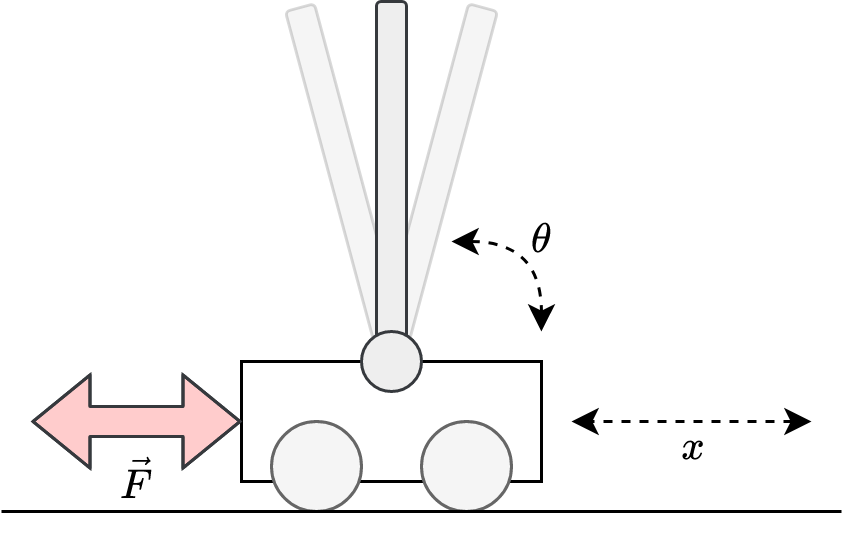
\includegraphics[width=.6\textwidth]{publications/2022CLEAVE/images/inverted_pendulum.png}
    \caption{
        The 2D inverted pendulum system.
    }\label{fig:invpend}
\end{figure}

\begin{figure}[t]
    \centering
    \begin{subfigure}[h]{.22\textwidth}
        \centering
        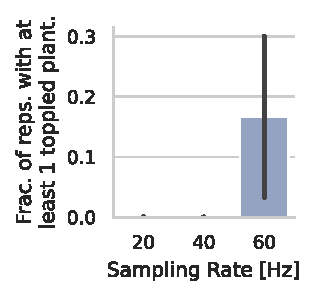
\includegraphics[width=\textwidth]{publications/2022CLEAVE/plots/fixed_video_topple_frac}
        \caption{Toppled plants.}\label{fig:video:toppled}
    \end{subfigure}%
    \hfill%
    \begin{subfigure}[h]{.22\textwidth}
        \centering
        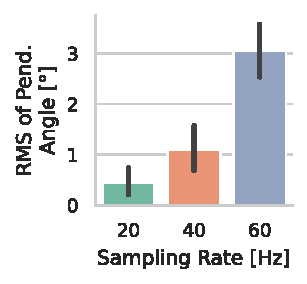
\includegraphics[width=\textwidth]{publications/2022CLEAVE/plots/fixed_video_angle_rms}
        \caption{Angle \ac{RMS}.}\label{fig:video:rms}
    \end{subfigure}\\
    \begin{subfigure}[h]{.22\textwidth}
        \centering
        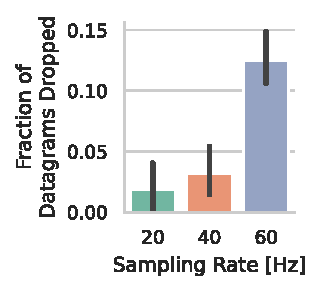
\includegraphics[width=\textwidth]{publications/2022CLEAVE/plots/fixed_video_drop_frac}
        \caption{Packet losses.}\label{fig:video:drop}
    \end{subfigure}%
    \hfill%
    \begin{subfigure}[h]{.22\textwidth}
        \centering
        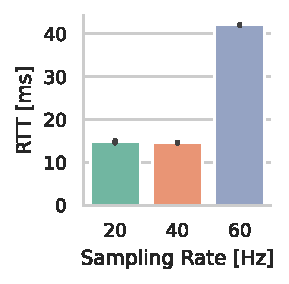
\includegraphics[width=\textwidth]{publications/2022CLEAVE/plots/fixed_video_rtt}
        \caption{\acsp{RTT}.}\label{fig:video:rtt}
    \end{subfigure}%
    \caption{
        Multi-loop, resource-constrained setup results.
        Error bars indicate \SI{95}{\percent} \acp{CI} in all plots.
    }\label{fig:video:results}
\end{figure}

\FloatBarrier%

\subsection{Orchestrating experimentation in edge computing testbeds}

\todo[inline]{\cref{paper:olguinmunoz2022ainur} describes a software framework for testbeds used for the methodology described in this thesis}

In this work, we present our solution to the challenge of testbed automation: Ainur, a framework for wireless testbed automation with a specific focus on end-to-end experimental research in the context of edge-computing using cloud- and edge-native technologies.
Ainur is designed to deploy experimental runs from a workload perspective by configuring the physical testbed, initializing all involved software components, deploying and executing the experimental workload, collecting logs and data, and finally gracefully degrading the system.
The framework allows for dynamic, software-definition of physical and logical links, network topology, cloud and edge computing resources, as well as experimental workload deployment and orchestration.
It heavily leverages cloud-native technologies, such as Docker containers, in order to support a wide variety of different testbed hardware setups and experimental configurations and workloads, as well as to be as easily extendable as possible.
Furthermore, we make Ainur available to the community as \ac{FOSS}.
It can be obtained from the {KTH-EXPECA/Ainur} repository on GitHub~\cite{ainur:github}, released under an Apache version \num{2.0} license.

In this paper, we have introduced a framework for repeatable end-to-end testbed automation in the context of wireless networking and edge computing research.
Named Ainur, it simplifies the execution and verification of end-to-end experimentation by automating the
\begin{enumerate*}[itemjoin={{; }}, itemjoin*={{; and }}]
    \item establishment of physical links between hosts, including the configuration of complex wireless systems such as 4G \ac{LTE} and 5G
    \item provisioning of and connection to remote cloud instances
    \item initialization of \ac{IP} layer connectivity between hosts
    \item collection of logs and data
    \item deployment, scaling, and lifecycle management of containerized processes
\end{enumerate*}.
We have described its general architecture, which follows a layered design mimicking the network stack layers the framework directly interacts with, as well as the underlying assumptions about its deployment environment and specific requirements for its deployment.
We have also outlined a demonstration which showcases the flexibility and power of the framework by deploying two different workloads to our testbed.
We believe our framework represents an important step towards repeatable, replicable, yet low-access barrier end-to-end wireless testbed experimentation.
It has been released as \ac{FOSS} and can be found on GitHub~\cite{ainur:github}.\\

\todo[inline]{Some plots}

\begin{figure}[t]
    \centering
    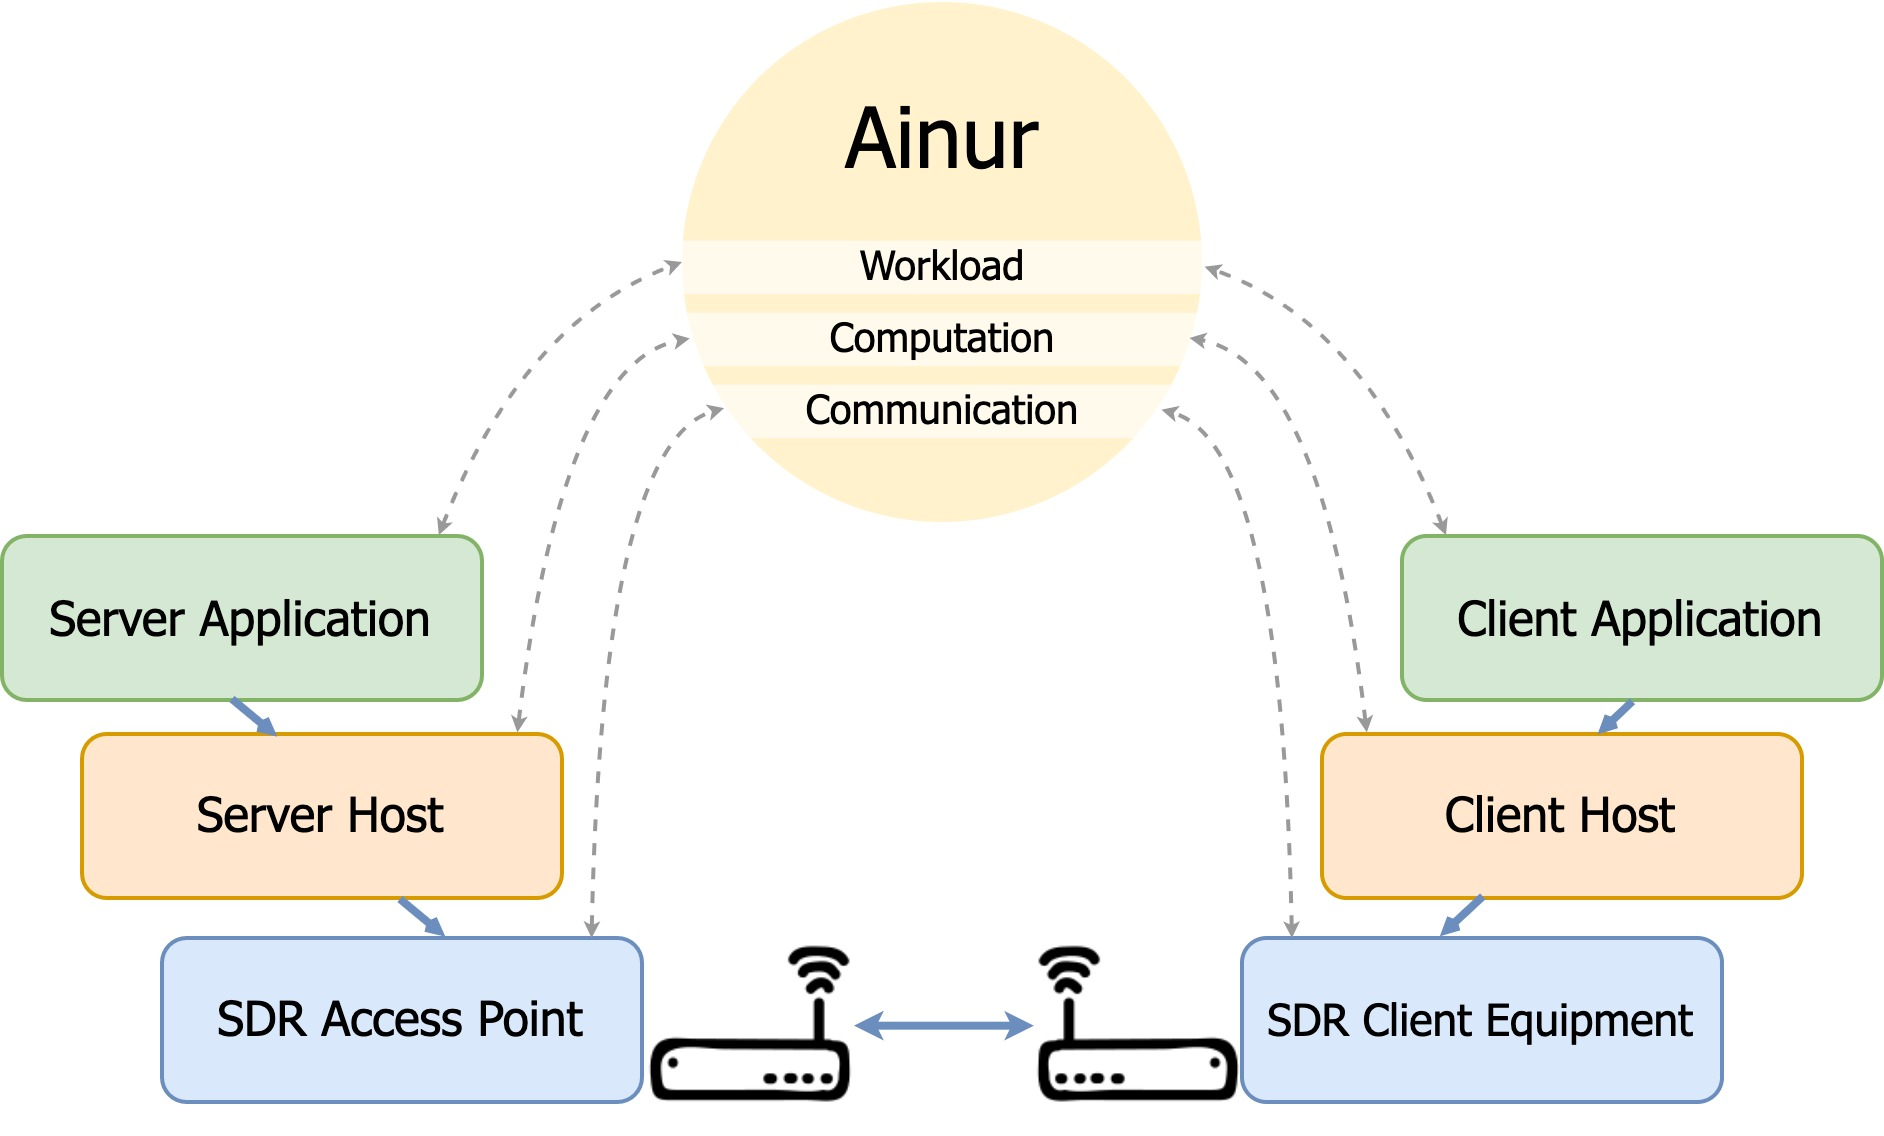
\includegraphics[width=0.9\linewidth]{publications/2022Ainur/figures/overview.jpg}
    \caption{Layered structure of an Ainur experiment}\label{fig:overview}
\end{figure}

\begin{figure*}
    \centering
    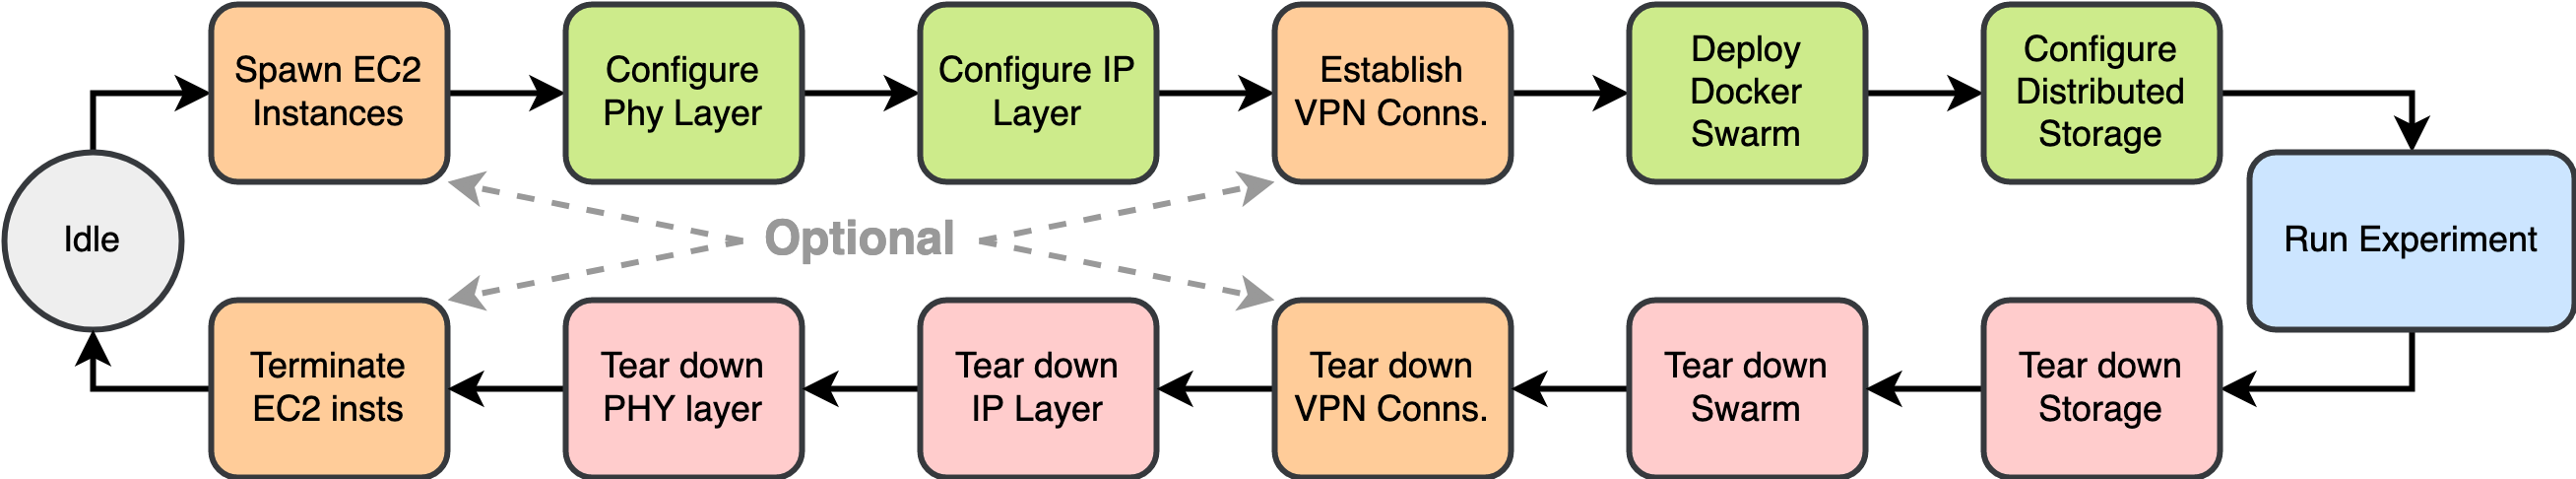
\includegraphics[width=0.8\textwidth]{publications/2022Ainur/figures/flow2.png}
    \caption{Lifecycle of an experimental run in Ainur. Blocks in orange are optional.}\label{fig:flow}
\end{figure*}

\begin{figure*}
    \centering
    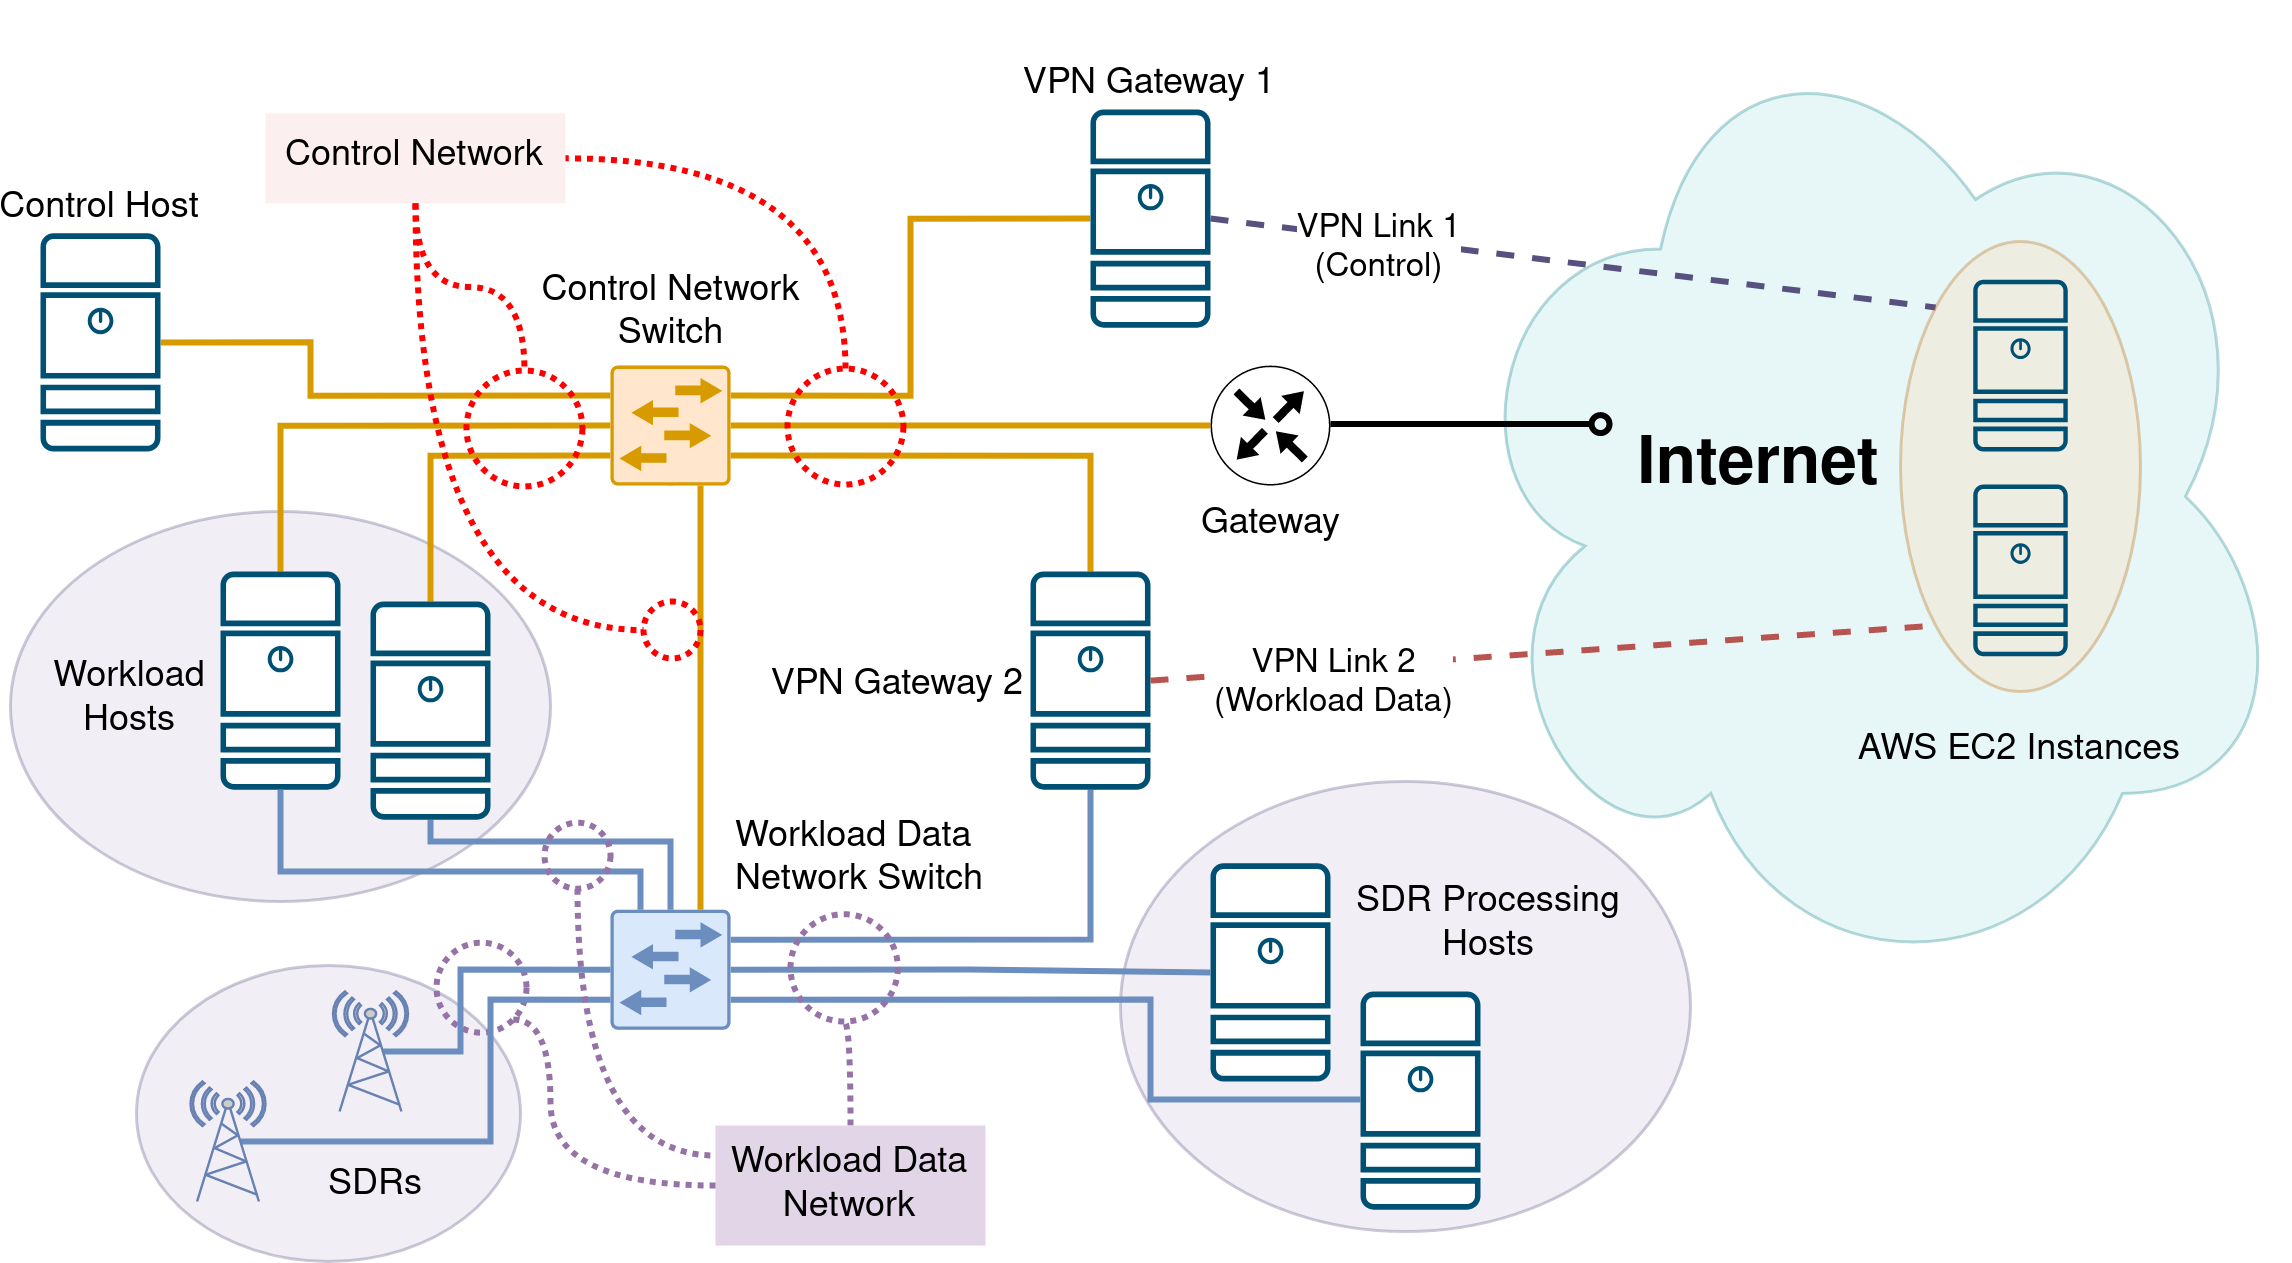
\includegraphics[width=.8\textwidth]{publications/2022Ainur/figures/network.png}
    \caption{Network structure assumed by Ainur.}\label{fig:network}
\end{figure*}

\section{Extending the methodology in the context of \acs{WCA}}

\subsection{Characterizing human behavior}

\todo[inline]{\cref{paper:olguinmunoz2021impact} describes the acquisition of the necessary data and insights for the models.}

\todo[inline]{From introduction}

We intended to answer four core research questions relating to human responses to decreased application responsiveness.

\begin{itemize}
    \item \emph{Do subjects change the temporal profile of their actions in relation to system latency?}

          In line with previous research in this area, we expected subjects to change their temporal profiles as system responsiveness decreased.
          The extent or form of these changes were however unknown.
          We also hypothesized that large enough drops in responsiveness could lead to complete abandonment of the task by subjects.

          Our results show an emergent pacing effect on user actions as system responsiveness is reduced.
          While it would seem self-evident that users take longer to complete a task while using a system with low responsiveness --- as they have to wait longer for new instructions --- our study found that user slow-down represents a source of substantial additional delay.
          To be more precise, the data indicate that users slow down not only because they have to wait for the system to catch up, but that their reactions to new instructions is also delayed.
          Moreover, this effect scales with the decrease in responsiveness and remains for a while, even after system responsiveness improves.

    \item \emph{Do subjects show signals of arousal in physiological responses to changes in system latency?}

          We hypothesized subjects would show signs of stress and frustration as system latency increased, due to the added annoyance of dealing with an unresponsive system.

          The results we present, however, seem to refute this hypothesis.
          We were not able to detect any significant effects on the physiological signals obtained from the biometric sensors as system responsiveness was altered.

    \item \emph{Are responses to delay effects in subjects mediated by cognition and/or emotion?}

          In line with previous items, we expected delay effects in subjects to be mediated primarily by emotion.
          In particular, we expected emotional effects to be correlated with the strength of the added delay.

          The results point in a different direction though, indicating that reduced responsiveness in WCA systems leads to a disruption of participants' cognitive plan for the task and not to an emotional response.
          This is evidenced by the previously discussed pacing effect and the lack of significant physiological responses.

    \item \emph{Are these effects mediated by personality indicators in any way?}

          Finally, we hypothesized that the individual trait of \emph{neuroticism}~\cite{john1999:bfi} would play a role in mediating these effects, as it has previously been connected to intolerance for time delay~\cite{hirsh2008delay}.
          We also expected \emph{focus} and \emph{involvement}~\cite{witmer1998:itq} to play roles in this.

          The results obtained agree with our hypothesis.
          We found significant effects of neuroticism on the responses exhibited by subjects, and all three traits were found to play a role through factor analysis.

\end{itemize}

% Our results indicate that reduced responsiveness in WCA systems leads to a disruption of participants' cognitive plan for the task.
% This is evidenced by an emergent pacing effect on user actions as system responsiveness is reduced.
% While it would seem self-evident that users take longer to complete a task while using a system with low responsiveness --- as they have to wait longer for new instructions --- our study found that user slow-down represents a source of substantial additional delay.
% To be more precise, the data indicate that users slow down not only because they have to wait for the system to catch up, but that their reactions to new instructions is also delayed.
% Furthermore, this effect persists for a while after system response improves and is modulated by intrinsic personality traits, in particular, \emph{neuroticism}~\cite{john1999:bfi}. 

We believe that these results provide concrete and relevant implications for WCA design, deployment, and optimization.
One example is the behavioral slow-down, as it extends application runtime significantly, and thus has clear and direct implications for resource and power consumption.
Another is the fact that the adverse effects of delay on users do not immediately subside as delay is diminished --- this has potential consequences for resource allocation strategies.
Moreover, in multi-user scenarios, the dependency of user slow-down effects on delay mean efficient resource allocation across applications potentially looks different from what could be considered ``fair''.

Our hope is that the results we provide might prove useful for the understanding and optimization of deployments of WCA.\@
These results represent unexpected, valuable findings, which can be employed to model and understand how users interact with latency in applications and systems, and develop resource allocation and power optimization strategies.
Additionally, we hope that the results we provide might pave the way for the improvement of performance evaluation tools such as our previous work in \cite{olguin:2018, olguin:2019}.
Such systems would greatly benefit from this knowledge, as it would allow for the design and implementation of realistic models of human behavior, making highly accurate benchmarks a reality in the domain of WCA.\@

\todo[inline]{From discussion}

We start our discussion with the main results of our experimentation presented in the previous section:

\begin{itemize}
    \item Firstly, and perhaps most importantly, we find that a system slow-down induces an \textit{additional} behavioral slow-down.
          That is, as system responsiveness decreases, our data indicates that users significantly slow-down in their execution of the task.
          This slow-down scales with the decrease in responsiveness; compared to the no-delay case, participants were on average \SI{12}{\percent} slower at \SI{1.65}{\second} delay and \SI{26}{\percent} at \SI{3.0}{\second} delay.
          Moreover, there is a temporal component to this effect; users become progressively slower the more time passes with reduced system responsiveness.

    \item Secondly, we find that the effects of behavioral slow-down due to impaired system responsiveness \emph{remain} for at least a few steps after system responsiveness improves.
          This is evidenced by the longer per-step-execution times of the first four steps of blocks immediately following a high-delay block, as pictured in \cref{fig:exectime:transition}.
          The question of whether any lingering effect can be measured after these four steps remains open.

    \item Thirdly, we evidence a speed-up in execution time over a series of steps; that is, subjects get faster at performing steps as the task progresses.
          However, the strength of this effect decreases as delay increases.
          Whereas for blocks without delay users performed the last four steps of a 12-step block on average \SI{36}{\percent} faster than the first four, at the maximum delay this effect practically disappears.

    \item Fourthly, in terms of inter-subject differences, PCA revealed three main factors governing users' response to delay.
          The first factor represents sensitivity to delay as moderated by the ``Big Five'' personality trait of neuroticism and both measures of immersion: focus and involvement.
          Factor two and three represent dedication to the task as opposed to delay intolerance and reflect variables related to attentiveness, respectively.
          In simple terms, these results suggest that the effects of delay are most potent in individuals who are sensitive and involved in the task.
          The findings appear selective to cognitive assistance tasks like the present ones, inasmuch as the same measures did not correlate with outcomes in other computer-intensive environments such as immersive VR~\cite{quesnel2018you}.
          These correlations are also consistent with previous findings indicating that individuals scoring high in neuroticism tend to be intolerant to delayed reward~\cite{hirsh2008delay}.
\end{itemize}

A central question therefore arises: to which physio- and psychological mechanisms can these findings, most importantly the substantial slow-down in task execution, be attributed?

In \cref{sec:background}, we initially considered the possibility that delays might produce negative emotional reactions.
These could in turn elicit generalized arousal.
We also postulated that adapting to delay might progressively deplete cognitive resources in users.
However, the present data provide relatively little support for these alternatives, in that the predicted measures did not produce the expected statistical trends.
Specifically, physiological measures of GSR and HR failed to show evidence of differential arousal under long vs.\ short delays, and speed-induced errors and non-completions predicted by resource depletion were not observed.
The acceleration data further did not indicate that extended delay significantly increases erratic movement.
% physiological measures of GSR and HR failed to show evidence of differential arousal under long vs.\ short delays, and speed-induced errors and non-completions predicted by resource depletion were not observed.
% The acceleration data further do not indicate that extended delay increases erratic movement.
To the contrary, the data suggest this effect results from a delay in movement after an instruction is introduced.
That is, users fail to capitalize on the new information as quickly as they could.
Thus, contrary to our preliminary postulations, behavioral effects seem to arise from impaired cognitive control mechanisms, and not from emotion or resource depletion.
We hypothesize that the effects of feedback latency can best be understood as changes in the use of a cognitive plan.
As was described in \cref{sec:experimentaldesign,fig:lego:hierarchical}, complex cognitive and motor tasks have been modeled as the unfolding of a hierarchy of command, from high-level plans to physical output.
Long system latencies, we propose, disrupt the automating of such a plan, instead relegating it to attention-based control at the step-by-step level that is easily diverted.
This also provides a possible explanation for the lingering effects of delay after an acceptable system responsiveness is restored, as users needs time re-adjust and re-automate their cognitive plans.

As to the applicability of our findings to other applications, it must be noted that these results pertain to a specific class of applications, namely step-based task-guidance WCA.\@
However, we would expect our findings to extend to similar applications, as long as they follow the same pattern of seamless interaction --- i.e.\ such that the user does not need explicitly interact with the application to advance the state.

The results here presented provide a number of possible implications for WCA system design and optimization, both for single and multi-application flows.

\begin{itemize}

    \item Due to the behavioral slow-down in users, even short-term reductions in responsiveness will lead to significantly extended application lifetimes.
          This has direct implications for resource and power consumption.

    \item The fact that the adverse effects of delay on users do not immediately disappear as the system returns to a high-responsive state could have unconventional consequences for resource allocation.
          This is of particular importance, for instance, for cases where the user may be able to finish the task before these effects subside.
          In such cases, the limited potential gains might not justify diverting valuable system resources to the impaired application.

    \item In multi-user environments, the time dependency of user slow-down effects mean that fair degradation of system responsiveness across applications may not ultimately be beneficial to the system as a whole.
          Take for instance two applications on the same system which negatively interfere with each other.
          The longer they interfere with each other, the longer their respective lifetimes are going to be, which in turn causes them to interfere even longer, potentially entering a positive feedback loop.
          In such a case, prioritizing one over the other rather than trying to improve responsiveness for both might lead to resources being freed up faster system-wide.

    \item Based on our findings relating individual differences between users and their sensitivity to delays, it might also be possible to extrapolate user characteristics from measured execution times.
          This could prove a valuable tool for load balancing, for instance by prioritizing resource allocation to users with a higher sensitivity to system-state degradation.
          However, this remains an open challenge.

\end{itemize}

To wrap up, we believe the present data provide novel and unexpected insights for the understanding and optimizing of WCA deployments.
Although more subtle than expected, and in some cases somewhat counterintuitive, these insights represent a valuable tool to tackle inefficiencies in these systems.
Moreover, we also argue these findings represent a first step towards a full-fledged understanding of the relationship between application responsiveness and human behavior.
More research in this area will surely uncover more complex and interesting behaviors.
Finally, we believe the data provide parameters that can usefully be integrated into cognitive models of WCA that might be constructed under existing architectures like ACT-R.
These same parameters could be used to modulate the timing and generation of inputs in trace-based workload generation tools such as the EdgeDroid platform~\cite{olguin:2018,olguin:2019}, allowing the tool to use the same trace to generate workloads for a multitude of different user profiles.

\todo[inline]{Some diagrams, plots, and results}

\begin{figure}[h]
    \centering
    \begin{subfigure}[t]{.49\textwidth}
        \centering
        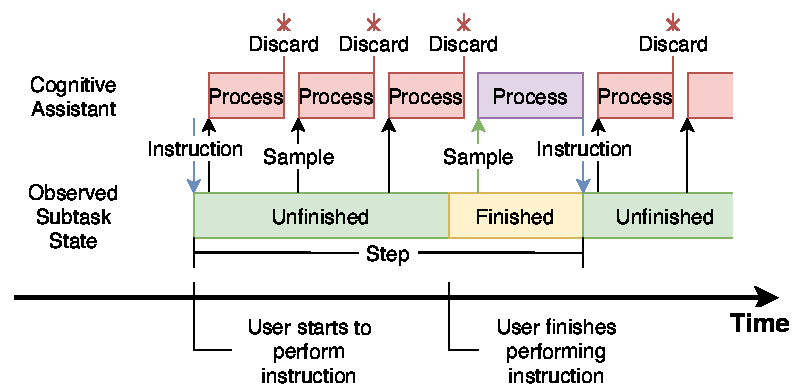
\includegraphics[width=\textwidth]{publications/2021ImpactDelayedResponse/Fig4a.eps}
        \caption{Structure of a step in a generic cognitive assistance application.
            The assistant provides an instruction to the user and continuously samples the step state; inputs captured while the step is unfinished are silently ``discarded'' (i.e.\ they do not cause the generation of a new instruction).
            % by the assistant, as they do not contain relevant information.
            Once the user finishes performing the step, the next sample \emph{will} cause the generation of a new instruction.
            % which will subsequently be provided to the user.}%
        }
        \label{fig:cogassist:step}
    \end{subfigure}%
    % \medskip%
    \hfill%
    \begin{subfigure}[t]{.49\textwidth}
        \centering
        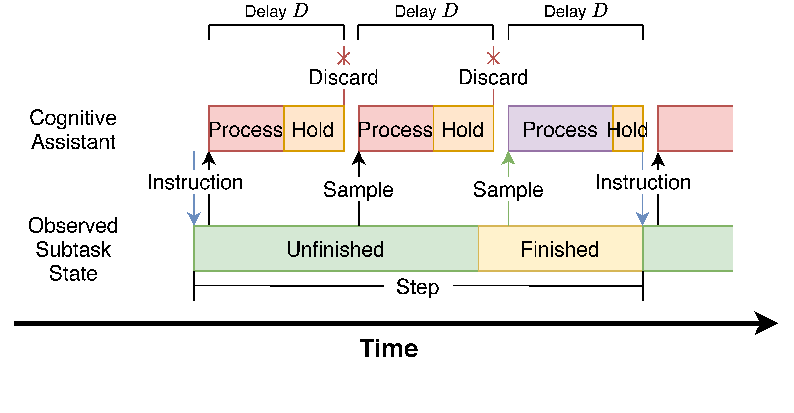
\includegraphics[width=\textwidth]{publications/2021ImpactDelayedResponse/Fig4b.eps}
        \caption{In the experimental task, an additional variable segment of time is introduced immediately following the processing of the input frame in order to extend the perceived processing time of the input to a specific target delay.}%
        \label{fig:cogassist:step:delay}
    \end{subfigure}
    \medskip%
    \begin{subfigure}[t]{.49\textwidth}
        \centering
        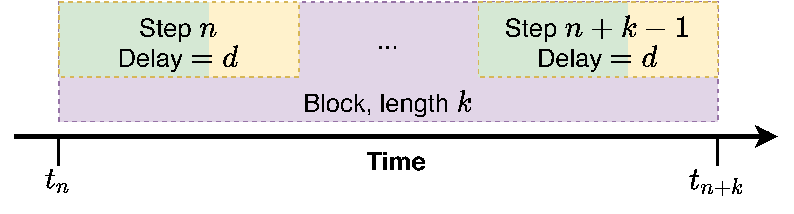
\includegraphics[width=\textwidth]{publications/2021ImpactDelayedResponse/Fig4c.eps}
        \caption{Structure of a block in the experimental task.}%
        \label{fig:cogassist:block}
    \end{subfigure}%
    % \medskip%
    \hfill%
    \begin{subfigure}[t]{.49\textwidth}
        \centering
        \includegraphics[width=\textwidth]{publications/2021ImpactDelayedResponse/Fig4d.eps}
        \caption{Visualization of the execution time of a step.}%
        \label{fig:exectime:diagram}
    \end{subfigure}%
    % \medskip%
    \caption{Components of the cognitive assistance task.}
\end{figure}

\begin{figure}[h]
    \centering
    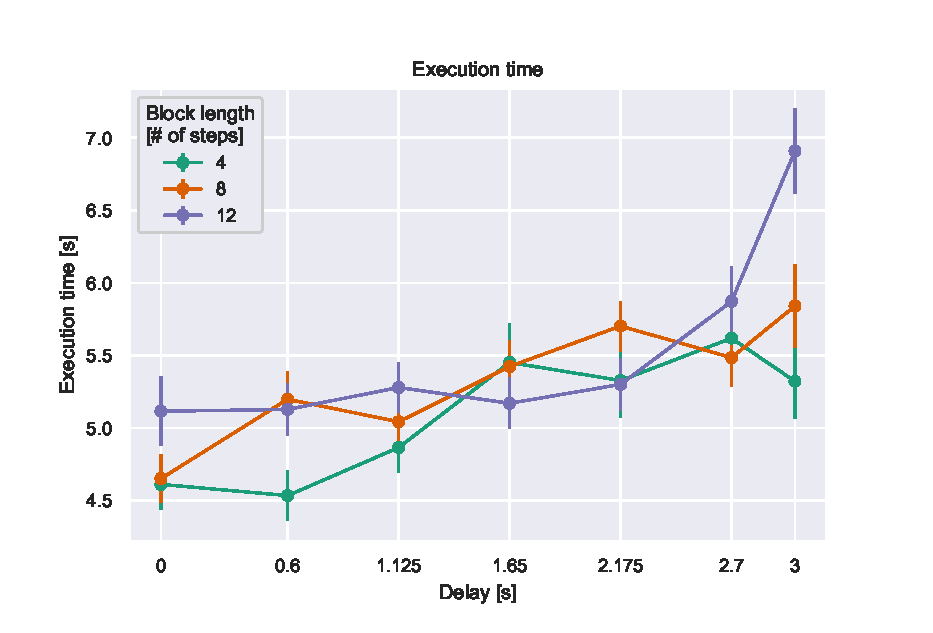
\includegraphics[width=.8\textwidth]{publications/2021ImpactDelayedResponse/Fig6.eps}
    \caption{Per-step execution time by block length vs.\ delay. Error bars indicate the Standard Error of the Mean (S.E.M.)}\label{fig:exectime}%    
\end{figure}

\begin{figure}[h]
    \centering
    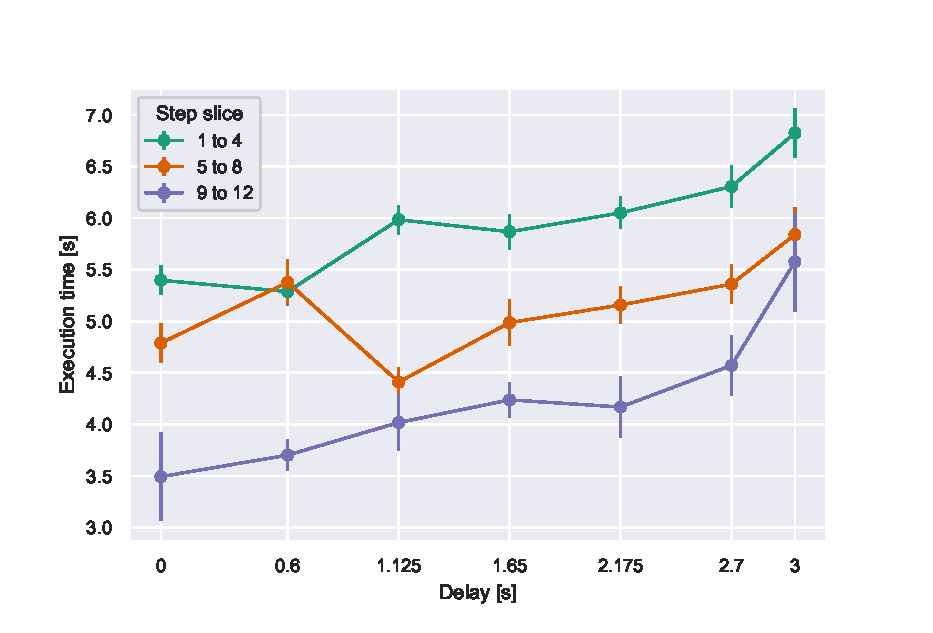
\includegraphics[width=.8\textwidth]{publications/2021ImpactDelayedResponse/Fig7.eps}
    \caption{Mean per-step execution time vs.\ delay, by step slice.
        Error bars indicate S.E.M.}
    \label{fig:exectime:delay:slice}
\end{figure}

\begin{figure}[h]
    \centering
    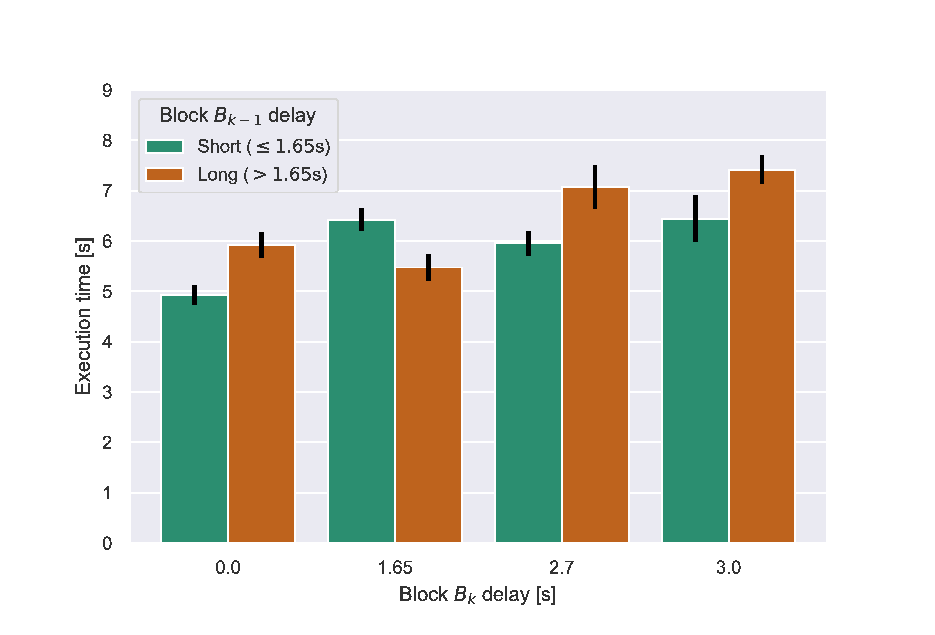
\includegraphics[width=.8\textwidth]{publications/2021ImpactDelayedResponse/Fig8.eps}
    \caption{Per-step execution time across the first four steps after a block transition from block \( B_{k-1} \) to \( B_k \). Error bars indicate S.E.M.}\label{fig:exectime:transition}%
\end{figure}

\begin{table}[h]
    \centering
    \caption{Principal Component Analysis}\label{tab:pca}
    \begin{subtable}[h]{\textwidth}
        \centering
        \caption{Main components identified.}
        \setlength{\tabcolsep}{0pt} % let TeX compute the intercolumn space
        \begin{tabular*}{\textwidth}{@{\extracolsep{\fill}\quad}lrrr@{}}
            \toprule
            \textbf{Factor} & \textbf{Comp. 1} & \textbf{Comp. 2} & \textbf{Comp. 3} \\
            \midrule
            BFI Conscientiousness                  & \textcolor{lightgray}{\( -0.022 \)} &                         \( 0.668 \) & \textcolor{lightgray}{\( -0.481 \)} \\
            BFI Neuroticism                        &                         \( 0.600 \) &                        \( -0.678 \) & \textcolor{lightgray}{\( -0.118 \)} \\
            ITQ Focus                              &                         \( 0.678 \) &  \textcolor{lightgray}{\( 0.203 \)} &                         \( 0.504 \) \\
            ITQ Involvement                        &                         \( 0.573 \) &                         \( 0.540 \) &  \textcolor{lightgray}{\( 0.417 \)} \\
            Exec. Time (delay 3.0 s, length 12)    &                         \( 0.758 \) & \textcolor{lightgray}{\( -0.178 \)} & \textcolor{lightgray}{\( -0.348 \)} \\
            Log EEG power \( \alpha + \beta \) Slice 1 & \textcolor{lightgray}{\( -0.436 \)} & \textcolor{lightgray}{\( -0.251 \)} &                         \( 0.589 \) \\
            \bottomrule
        \end{tabular*}
    \end{subtable}
    \newline
    \medskip
    \newline
    \begin{subtable}[h]{\textwidth}
        \centering
        \caption{Percentages of variance explained by the components.}
        \begin{tabular*}{\textwidth}{@{\extracolsep{\fill}\quad}lrrrr@{}}
            \toprule
            {} & \textbf{Comp. 1} & \textbf{Comp. 2} & \textbf{Comp. 3} & \textbf{Total} \\
            \midrule
            Explained Variance & \SI{31.88}{\percent} & \SI{22.22}{\percent} & \SI{19.03}{\percent} & \SI{73.13}{\percent} \\
            \bottomrule
        \end{tabular*}
    \end{subtable}
\end{table}

\subsection{Emulating human behavior}

We introduce the first, to our knowledge, data-driven model for human timings in \ac{WCA} applications.
Using the data collected for \textcite{olguinmunoz:impact2021} as a base, we build a stochastic model which takes as input past measurements of system responsiveness and produces realistic step execution times.
We also introduce a novel way to generate dynamic traces of frames for \ac{WCA} applications which can be combined with the timing model for a full end-to-end emulation of a human.
We name this new model \emph{EdgeDroid 2.0}; a direct, more realistic evolution of our initial EdgeDroid approach~\cite{olguin2018scaling,olguin2019edgedroid}.

The study and benchmarking of \ac{WCA} applications is a challenging discipline due to these application's intrinsic human-in-the-loop nature.
Humans are notoriously unreliable, and greatly complicate the scalability and repeatability of experiments.
Furthermore, recruiting large enough cohorts of humans for large-scale experimentation is both greatly time-consuming and prohibitively expensive for many research groups.

In the first half of this paper, we have introduced the EdgeDroid 2.0 model of human timing behavior for \ac{WCA}, the first data-driven model for human timings in \ac{WCA} applications.
This model represents a stochastic approach to execution time modeling which builds upon the data collected for \textcite{olguinmunoz:impact2021}.
Together with this model, we have also introduced a novel procedure for the generation of synthetic traces of frames in step-based \ac{WCA}, allowing for a full end-to-end emulation of a human when combined with the timing model.

\todo[inline]{TODO: Some relevant results. Need to add paper to thesis.}

\section{Implications for the optimization of \ac{WCA}}

\begin{enumerate}
    \item\label{item:contrib:footprint} Using the model described above, we study the implications of realistic human behavior on the application lifetime footprint of \ac{WCA}.
    In concordance with previous work~\cite{olguinmunoz:impact2021}, we find dependencies between system responsiveness and human step execution times that lead to substantially different application lifetimes when compared to a first-order baseline which does not take into account human behavior.
    \item\label{item:contrib:optimization} Finally, we study the potential for optimization in \ac{WCA} when considering human behavior using our model.
    We develop a generic model for the stochastic optimization of resource consumption versus responsiveness trade-offs in these applications, which we apply to two potential avenues for \ac{WCA} optimization; number of processed samples and energy consumption per step.
    Compared to the state-of-the-art, our optimization model results in up to \textasciitilde\SI{60}{\percent} fewer samples processed or an average of \SI{20}{\percent} less energy consumed per step, while maintaining comparable levels of responsiveness.
\end{enumerate}

Next, we have explored the impact of such a realistic model on the application lifetime footprint of \ac{WCA} applications.
We have shown that less realistic modeling approaches which do not take into account higher-order effects on execution time distributions can potentially lead to significant misestimations of application footprint.

Finally, we have delved into the potential for optimization in \ac{WCA} systems using the previously discussed timing models.
We have proposed a novel stochastic optimization framework for resource consumption-system responsiveness trade-offs in \ac{WCA} which results in an adaptive sampling strategy.
We have shown that this framework is applicable to a myriad of metrics in these applications, and showcased experimental results employing this framework for the minimization of number of samples processed per step and total energy consumption per step.
Our results show up to a \SI{50}{\percent} increase in performance with respect to state of the art when optimizing for number of samples, and up to a \SI{30}{\percent} improvement when optimizing for energy consumption, proving thus the value of such frameworks for the design of \ac{WCA} applications.

\chapter{Conclusions}
% %------------------------------------------------
% % CREATING THE BIBLIOGRAPHY
% %------------------------------------------------
% \bibliographystyle{ieeetr}
% \renewcommand{\bibname}{References}% changes default name Bibliography to References
% \bibliography{../Refs} % References file

% %--------------------------------------------------

\nocite{*}
\printbibliography[
    heading=bibintoc,
    title=References,
    notcategory=thesispapers
]{}

\part{Publications}

\end{document}
\endinput
%%
%% End of file `kth-demo.tex'.
